\section{zesto-cache.cpp File Reference}
\label{config_2zesto-cache_8cpp}\index{zesto-cache.cpp@{zesto-cache.cpp}}
{\tt \#include $<$limits.h$>$}\par
{\tt \#include \char`\"{}thread.h\char`\"{}}\par
{\tt \#include \char`\"{}stats.h\char`\"{}}\par
{\tt \#include \char`\"{}zesto-core.h\char`\"{}}\par
{\tt \#include \char`\"{}zesto-opts.h\char`\"{}}\par
{\tt \#include \char`\"{}zesto-cache.h\char`\"{}}\par
{\tt \#include \char`\"{}zesto-prefetch.h\char`\"{}}\par
{\tt \#include \char`\"{}zesto-uncore.h\char`\"{}}\par
{\tt \#include \char`\"{}zesto-exec.h\char`\"{}}\par
{\tt \#include \char`\"{}zesto-commit.h\char`\"{}}\par


Include dependency graph for config/zesto-cache.cpp:\nopagebreak
\begin{figure}[H]
\begin{center}
\leavevmode
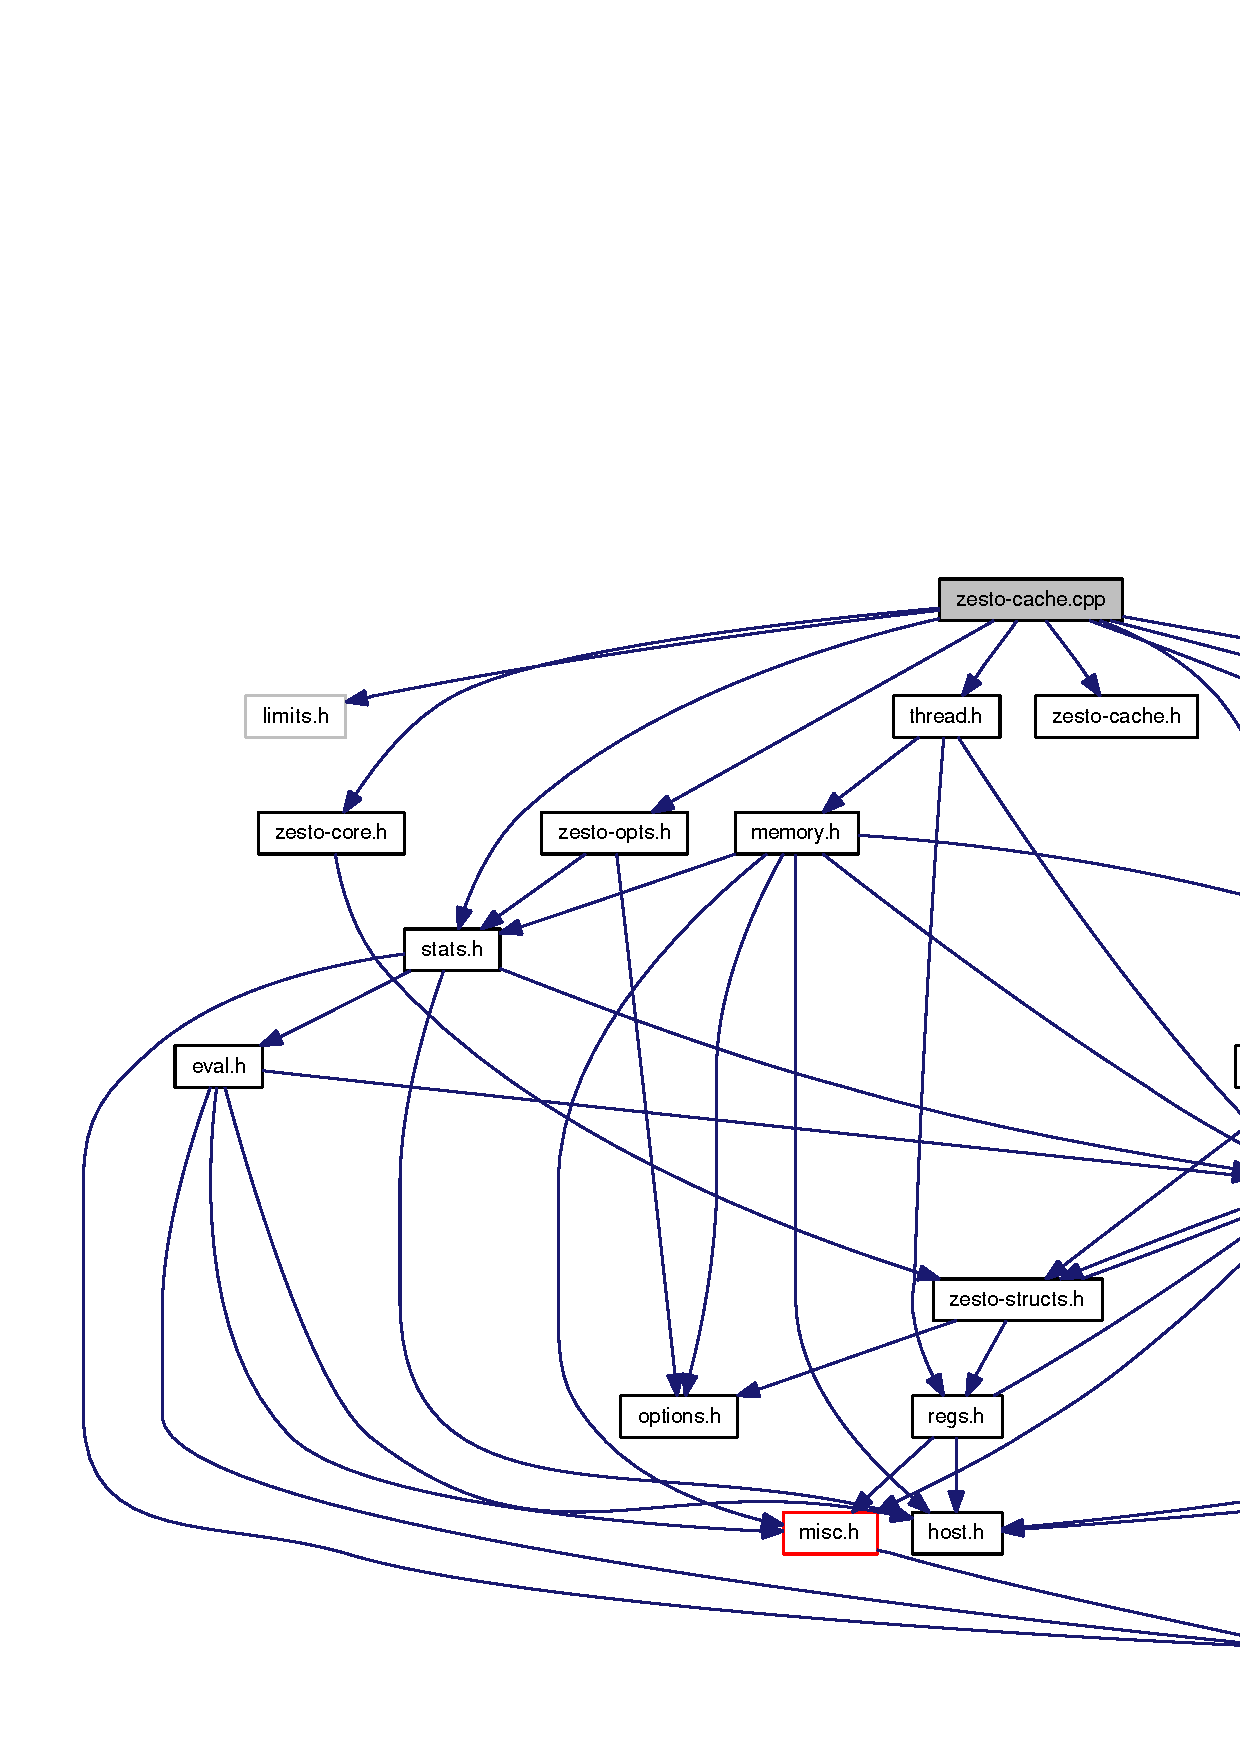
\includegraphics[width=420pt]{config_2zesto-cache_8cpp__incl}
\end{center}
\end{figure}
\subsection*{Functions}
\begin{CompactItemize}
\item 
struct {\bf cache\_\-t} $\ast$ {\bf cache\_\-create} (struct {\bf core\_\-t} $\ast$const core, const char $\ast$const name, const bool read\_\-only, const int sets, const int assoc, const int linesize, const char rp, const char ap, const char wp, const char wc, const int banks, const int bank\_\-width, const int latency, const int WBB\_\-size, const int MSHR\_\-size, const int MSHR\_\-banks, struct {\bf cache\_\-t} $\ast$const next\_\-level\_\-cache, struct {\bf bus\_\-t} $\ast$const next\_\-bus)
\item 
void {\bf cache\_\-reg\_\-stats} (struct {\bf stat\_\-sdb\_\-t} $\ast$const sdb, const struct {\bf core\_\-t} $\ast$const core, struct {\bf cache\_\-t} $\ast$const cp)
\item 
void {\bf cache\_\-reset\_\-stats} (struct {\bf cache\_\-t} $\ast$const cp)
\item 
void {\bf prefetch\_\-buffer\_\-create} (struct {\bf cache\_\-t} $\ast$const cp, const int num\_\-entries)
\item 
void {\bf prefetch\_\-filter\_\-create} (struct {\bf cache\_\-t} $\ast$const cp, const int num\_\-entries, const int reset\_\-interval)
\item 
static int {\bf prefetch\_\-filter\_\-lookup} (struct {\bf prefetch\_\-filter\_\-t} $\ast$const p, const {\bf md\_\-paddr\_\-t} addr)
\item 
static void {\bf prefetch\_\-filter\_\-update} (struct {\bf prefetch\_\-filter\_\-t} $\ast$const p, const {\bf md\_\-paddr\_\-t} addr, const int useful)
\item 
struct {\bf cache\_\-line\_\-t} $\ast$ {\bf cache\_\-is\_\-hit} (struct {\bf cache\_\-t} $\ast$const cp, const enum {\bf cache\_\-command} cmd, const {\bf md\_\-paddr\_\-t} addr, struct {\bf core\_\-t} $\ast$const core)
\item 
static struct {\bf cache\_\-line\_\-t} $\ast$ {\bf cache\_\-peek} (const struct {\bf cache\_\-t} $\ast$const cp, const {\bf md\_\-paddr\_\-t} addr)
\item 
void {\bf cache\_\-insert\_\-block} (struct {\bf cache\_\-t} $\ast$const cp, const enum {\bf cache\_\-command} cmd, const {\bf md\_\-paddr\_\-t} addr, {\bf core\_\-t} $\ast$const core)
\item 
struct {\bf cache\_\-line\_\-t} $\ast$ {\bf cache\_\-get\_\-evictee} (struct {\bf cache\_\-t} $\ast$const cp, const {\bf md\_\-paddr\_\-t} addr, {\bf core\_\-t} $\ast$const core)
\item 
static void {\bf cache\_\-heap\_\-balance} (struct {\bf cache\_\-action\_\-t} $\ast$const pipe, const int insert\_\-position)
\item 
static void {\bf cache\_\-heap\_\-remove} (struct {\bf cache\_\-action\_\-t} $\ast$const pipe, const int pipe\_\-num)
\item 
int {\bf cache\_\-enqueuable} (const struct {\bf cache\_\-t} $\ast$const cp, const int thread\_\-id, const {\bf md\_\-paddr\_\-t} addr)
\item 
void {\bf cache\_\-enqueue} (struct {\bf core\_\-t} $\ast$const core, struct {\bf cache\_\-t} $\ast$const cp, struct {\bf cache\_\-t} $\ast$const prev\_\-cp, const enum {\bf cache\_\-command} cmd, const int thread\_\-id, const {\bf md\_\-addr\_\-t} PC, const {\bf md\_\-paddr\_\-t} addr, const {\bf seq\_\-t} action\_\-id, const int MSHR\_\-bank, const int MSHR\_\-index, void $\ast$const op, void($\ast$const cb)(void $\ast$), void($\ast$const miss\_\-cb)(void $\ast$, int), bool($\ast$const translated\_\-cb)(void $\ast$, {\bf seq\_\-t}), {\bf seq\_\-t}($\ast$const get\_\-action\_\-id)(void $\ast$))
\item 
static int {\bf WBB\_\-available} (const struct {\bf cache\_\-t} $\ast$const cp, const {\bf md\_\-paddr\_\-t} paddr)
\item 
static void {\bf WBB\_\-insert} (struct {\bf cache\_\-t} $\ast$const cp, struct {\bf cache\_\-line\_\-t} $\ast$const cache\_\-block)
\item 
static void {\bf WBB\_\-victim\_\-insert} (struct {\bf cache\_\-t} $\ast$const cp, struct {\bf cache\_\-line\_\-t} $\ast$const cache\_\-block)
\item 
static int {\bf MSHR\_\-available} (const struct {\bf cache\_\-t} $\ast$const cp, const {\bf md\_\-paddr\_\-t} paddr)
\item 
static struct {\bf cache\_\-action\_\-t} $\ast$ {\bf MSHR\_\-allocate} (struct {\bf cache\_\-t} $\ast$const cp, const {\bf md\_\-paddr\_\-t} paddr, const enum {\bf cache\_\-command} cmd)
\item 
static void {\bf dummy\_\-callback} (void $\ast$p)
\item 
void {\bf fill\_\-arrived} (struct {\bf cache\_\-t} $\ast$const cp, const int MSHR\_\-bank, const int MSHR\_\-index)
\item 
void {\bf print\_\-heap} (const struct {\bf cache\_\-t} $\ast$const cp)
\item 
static void {\bf fill\_\-heap\_\-balance} (struct {\bf cache\_\-fill\_\-t} $\ast$const pipe, const int insert\_\-position)
\item 
static void {\bf fill\_\-heap\_\-remove} (struct {\bf cache\_\-fill\_\-t} $\ast$const pipe, const int pipe\_\-num)
\item 
static bool {\bf cache\_\-fillable} (const struct {\bf cache\_\-t} $\ast$const cp, const {\bf md\_\-paddr\_\-t} paddr)
\item 
static void {\bf cache\_\-fill} (struct {\bf cache\_\-t} $\ast$const cp, const enum {\bf cache\_\-command} cmd, const {\bf md\_\-paddr\_\-t} paddr, struct {\bf core\_\-t} $\ast$core)
\item 
void {\bf cache\_\-process} (struct {\bf cache\_\-t} $\ast$const cp)
\item 
static void {\bf cache\_\-prefetch} (struct {\bf cache\_\-t} $\ast$const cp)
\item 
static void {\bf prefetch\_\-controller\_\-update} (struct {\bf cache\_\-t} $\ast$const cp)
\item 
void {\bf step\_\-core\_\-PF\_\-controllers} (struct {\bf core\_\-t} $\ast$const core)
\item 
void {\bf prefetch\_\-core\_\-caches} (struct {\bf core\_\-t} $\ast$const core)
\item 
void {\bf cache\_\-freeze\_\-stats} (struct {\bf core\_\-t} $\ast$const core)
\item 
void {\bf cache\_\-print} (const struct {\bf cache\_\-t} $\ast$const cp)
\item 
struct {\bf bus\_\-t} $\ast$ {\bf bus\_\-create} (const char $\ast$const name, const int width, const int ratio)
\item 
void {\bf bus\_\-reg\_\-stats} (struct {\bf stat\_\-sdb\_\-t} $\ast$const sdb, struct {\bf core\_\-t} $\ast$const core, struct {\bf bus\_\-t} $\ast$const bus)
\item 
int {\bf bus\_\-free} (const struct {\bf bus\_\-t} $\ast$const bus)
\item 
void {\bf bus\_\-use} (struct {\bf bus\_\-t} $\ast$const bus, const int transfer\_\-size, const int prefetch)
\end{CompactItemize}


\subsection{Function Documentation}
\index{config/zesto-cache.cpp@{config/zesto-cache.cpp}!bus\_\-create@{bus\_\-create}}
\index{bus\_\-create@{bus\_\-create}!config/zesto-cache.cpp@{config/zesto-cache.cpp}}
\subsubsection[{bus\_\-create}]{\setlength{\rightskip}{0pt plus 5cm}struct {\bf bus\_\-t}$\ast$ bus\_\-create (const char $\ast$const  {\em name}, \/  const int {\em width}, \/  const int {\em ratio})\hspace{0.3cm}{\tt  [read]}}\label{config_2zesto-cache_8cpp_cf58fdfdf1939cc2b0b05b50ac0eedd8}




Definition at line 2465 of file config/zesto-cache.cpp.

Referenced by core\_\-exec\_\-DPM\_\-t::core\_\-exec\_\-DPM\_\-t(), core\_\-exec\_\-STM\_\-t::core\_\-exec\_\-STM\_\-t(), and uncore\_\-t::uncore\_\-t().

Here is the caller graph for this function:\nopagebreak
\begin{figure}[H]
\begin{center}
\leavevmode
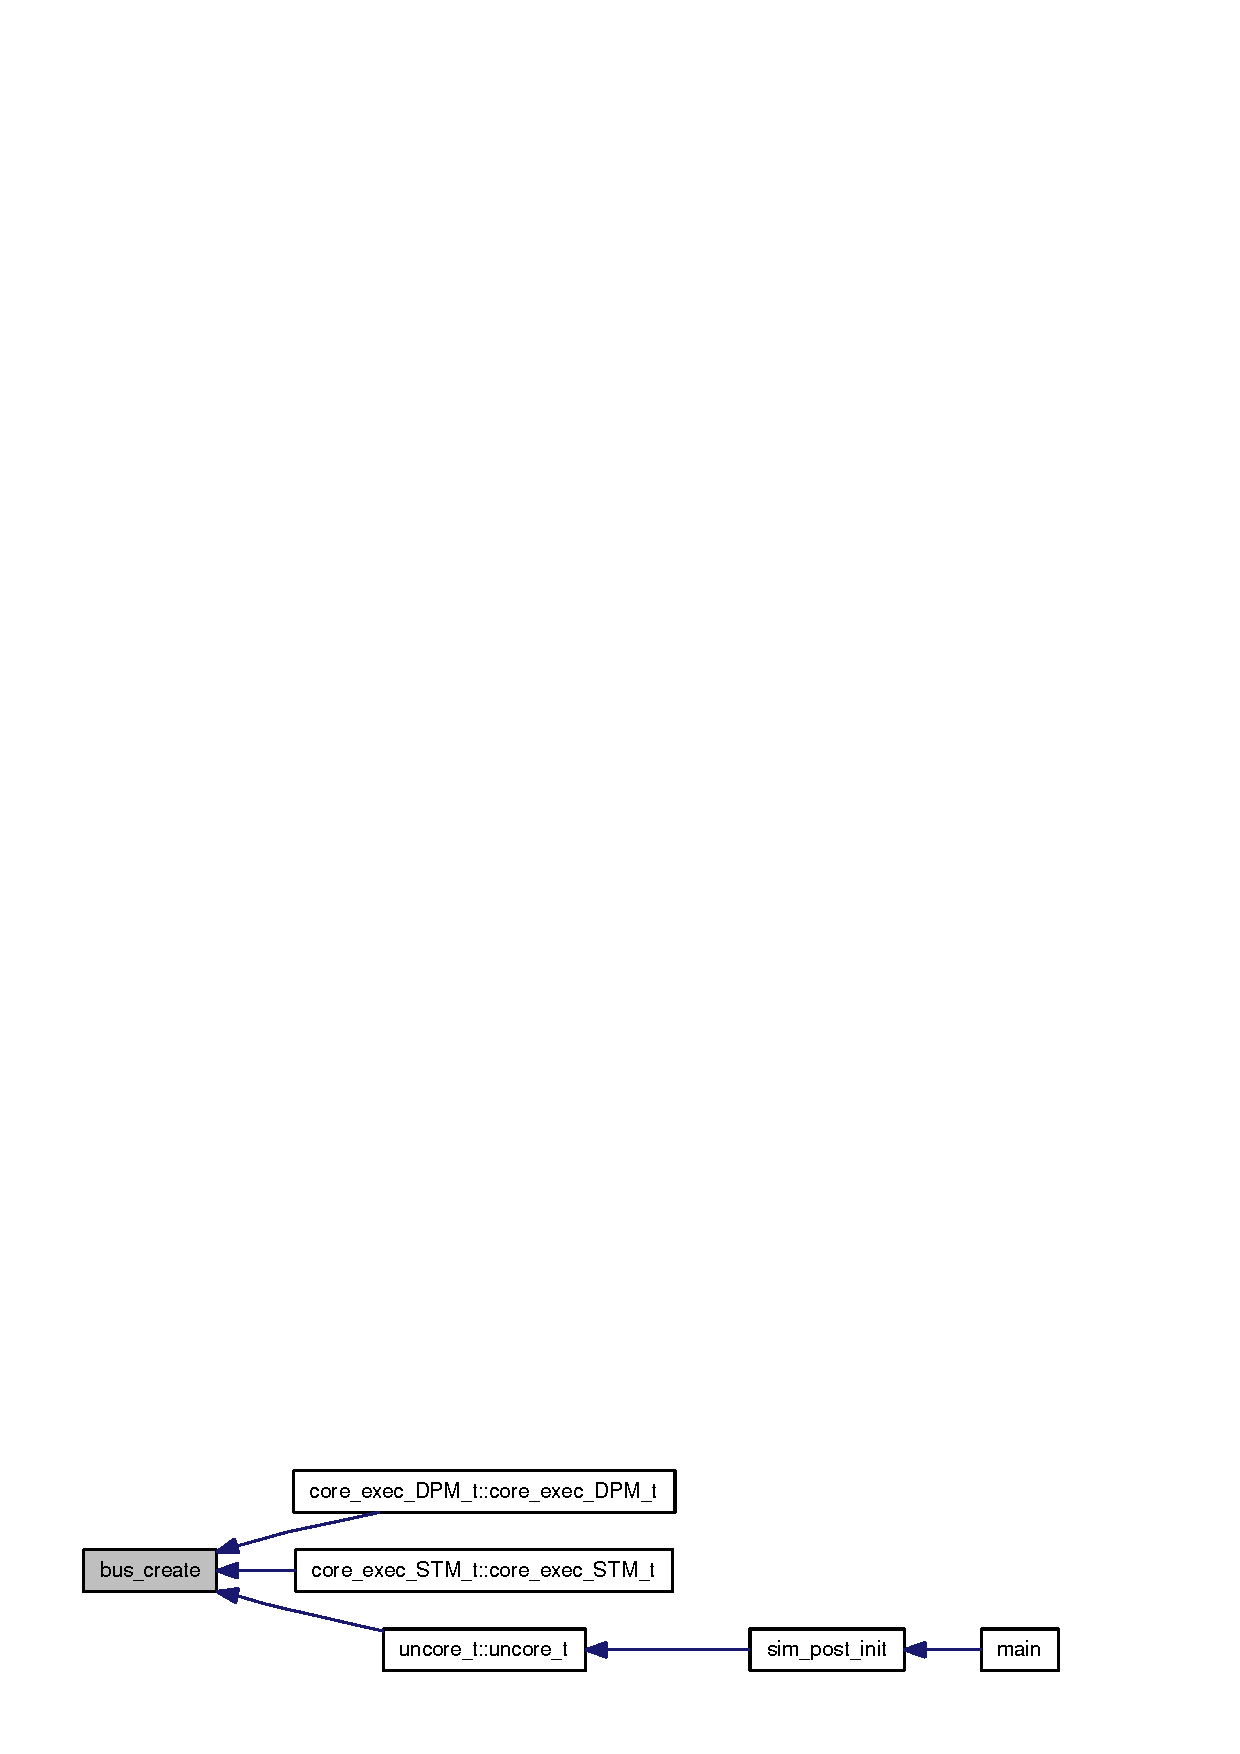
\includegraphics[width=256pt]{config_2zesto-cache_8cpp_cf58fdfdf1939cc2b0b05b50ac0eedd8_icgraph}
\end{center}
\end{figure}
\index{config/zesto-cache.cpp@{config/zesto-cache.cpp}!bus\_\-free@{bus\_\-free}}
\index{bus\_\-free@{bus\_\-free}!config/zesto-cache.cpp@{config/zesto-cache.cpp}}
\subsubsection[{bus\_\-free}]{\setlength{\rightskip}{0pt plus 5cm}int bus\_\-free (const struct {\bf bus\_\-t} $\ast$const  {\em bus})}\label{config_2zesto-cache_8cpp_24292dcf41327971f03a4c7150cbdf28}




Definition at line 2518 of file config/zesto-cache.cpp.

Referenced by cache\_\-process(), and cache\_\-process\_\-llc().

Here is the caller graph for this function:\nopagebreak
\begin{figure}[H]
\begin{center}
\leavevmode
\includegraphics[width=211pt]{config_2zesto-cache_8cpp_24292dcf41327971f03a4c7150cbdf28_icgraph}
\end{center}
\end{figure}
\index{config/zesto-cache.cpp@{config/zesto-cache.cpp}!bus\_\-reg\_\-stats@{bus\_\-reg\_\-stats}}
\index{bus\_\-reg\_\-stats@{bus\_\-reg\_\-stats}!config/zesto-cache.cpp@{config/zesto-cache.cpp}}
\subsubsection[{bus\_\-reg\_\-stats}]{\setlength{\rightskip}{0pt plus 5cm}void bus\_\-reg\_\-stats (struct {\bf stat\_\-sdb\_\-t} $\ast$const  {\em sdb}, \/  struct {\bf core\_\-t} $\ast$const  {\em core}, \/  struct {\bf bus\_\-t} $\ast$const  {\em bus})}\label{config_2zesto-cache_8cpp_22d7e9c4a1a2031601e5a3ad3694768c}




Definition at line 2479 of file config/zesto-cache.cpp.

Referenced by core\_\-exec\_\-STM\_\-t::reg\_\-stats(), and uncore\_\-t::uncore\_\-reg\_\-stats().

Here is the caller graph for this function:\nopagebreak
\begin{figure}[H]
\begin{center}
\leavevmode
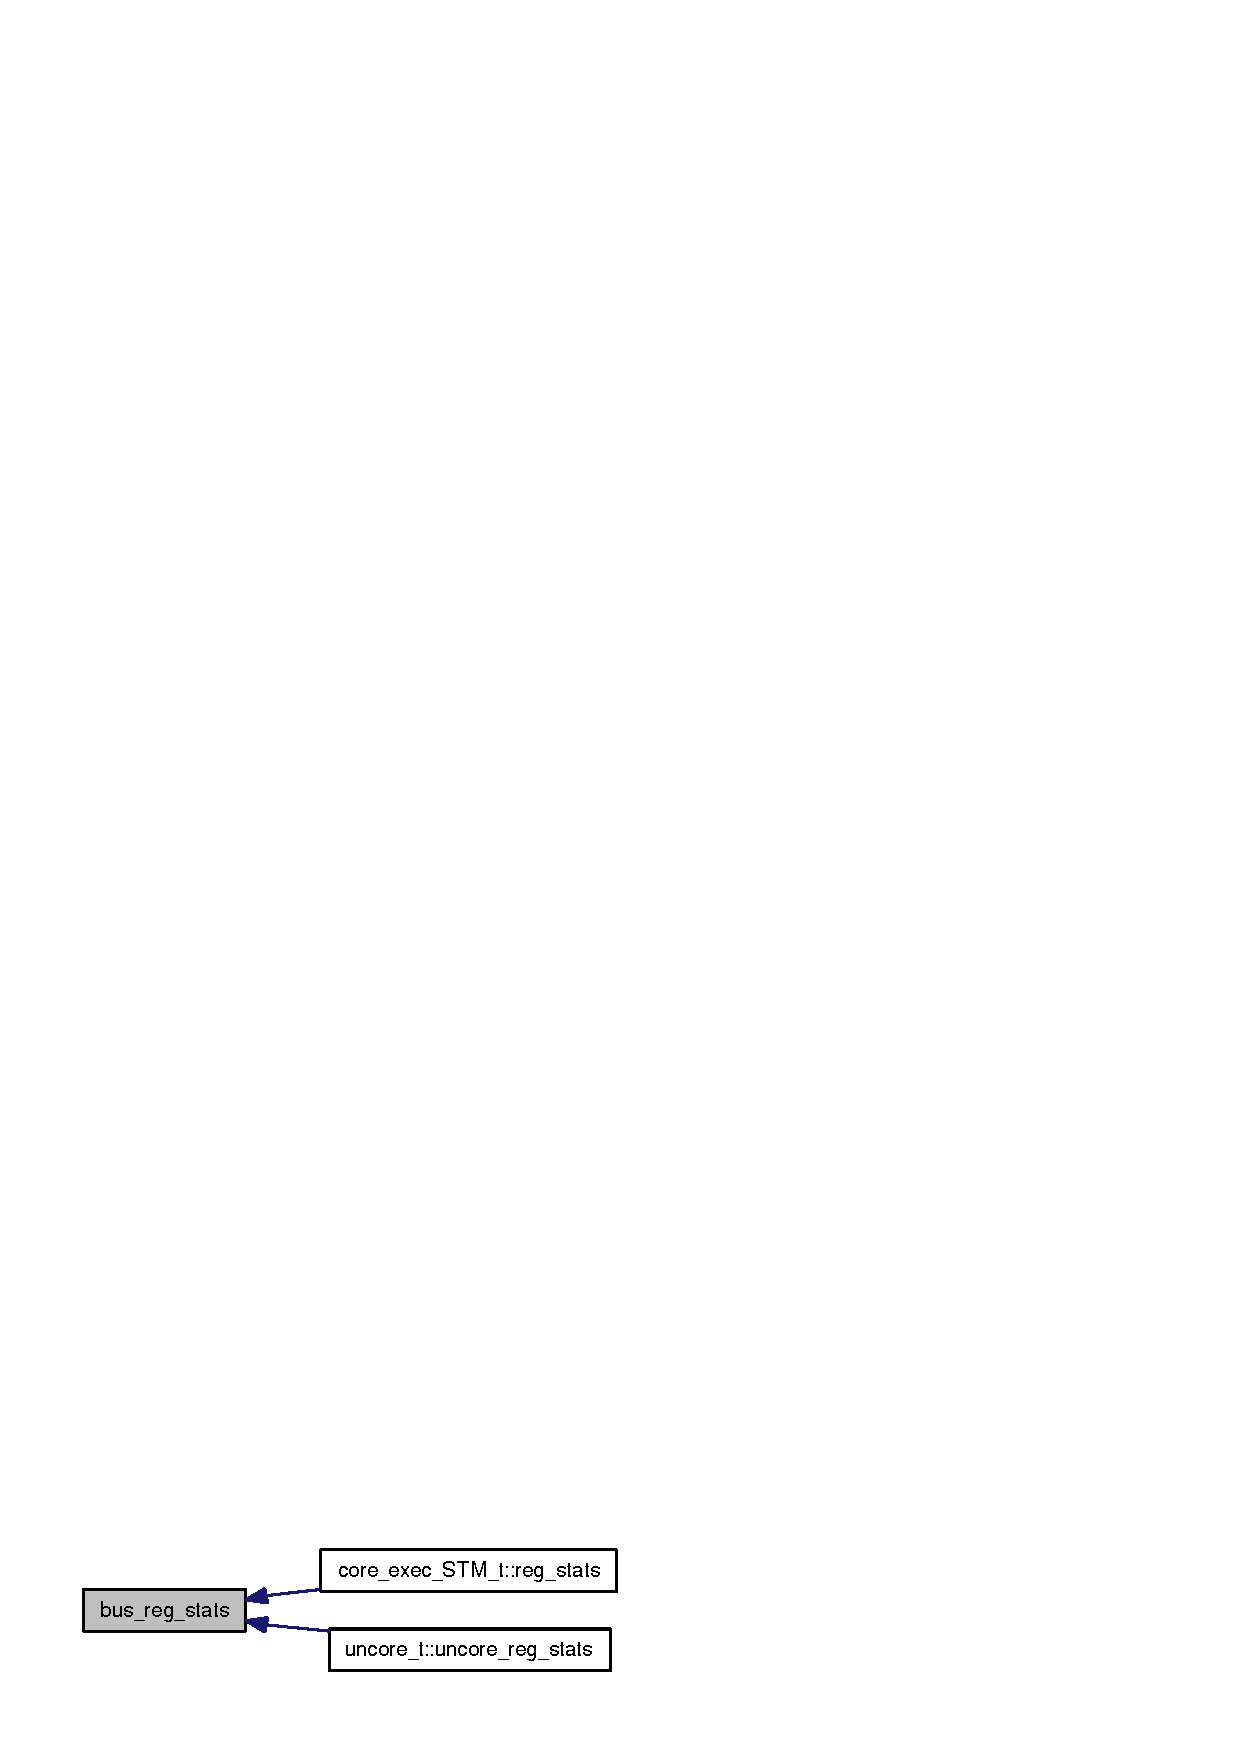
\includegraphics[width=150pt]{config_2zesto-cache_8cpp_22d7e9c4a1a2031601e5a3ad3694768c_icgraph}
\end{center}
\end{figure}
\index{config/zesto-cache.cpp@{config/zesto-cache.cpp}!bus\_\-use@{bus\_\-use}}
\index{bus\_\-use@{bus\_\-use}!config/zesto-cache.cpp@{config/zesto-cache.cpp}}
\subsubsection[{bus\_\-use}]{\setlength{\rightskip}{0pt plus 5cm}void bus\_\-use (struct {\bf bus\_\-t} $\ast$const  {\em bus}, \/  const int {\em transfer\_\-size}, \/  const int {\em prefetch})}\label{config_2zesto-cache_8cpp_cb6440bff7b9405665cbae0d836630f3}




Definition at line 2529 of file config/zesto-cache.cpp.

Referenced by cache\_\-process(), and cache\_\-process\_\-llc().

Here is the caller graph for this function:\nopagebreak
\begin{figure}[H]
\begin{center}
\leavevmode
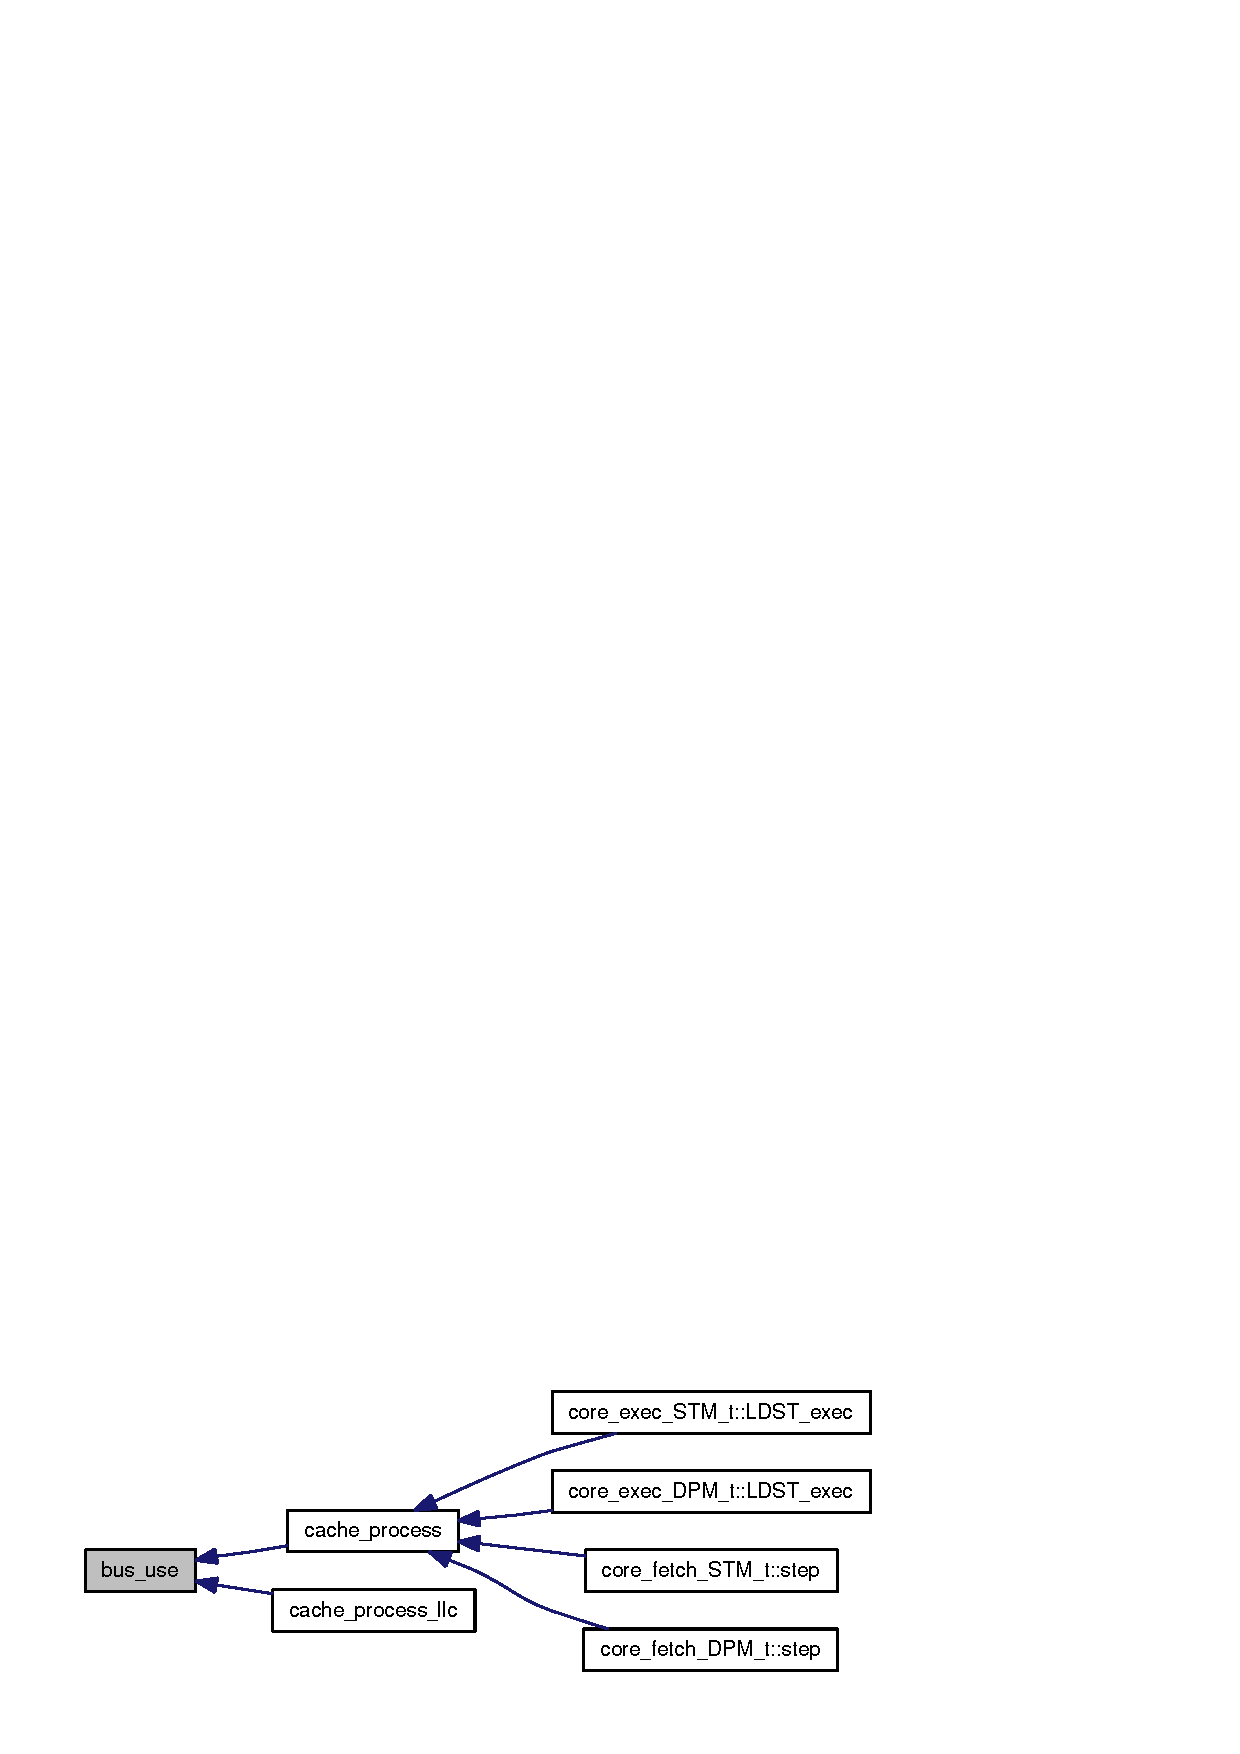
\includegraphics[width=211pt]{config_2zesto-cache_8cpp_cb6440bff7b9405665cbae0d836630f3_icgraph}
\end{center}
\end{figure}
\index{config/zesto-cache.cpp@{config/zesto-cache.cpp}!cache\_\-create@{cache\_\-create}}
\index{cache\_\-create@{cache\_\-create}!config/zesto-cache.cpp@{config/zesto-cache.cpp}}
\subsubsection[{cache\_\-create}]{\setlength{\rightskip}{0pt plus 5cm}struct {\bf cache\_\-t}$\ast$ cache\_\-create (struct {\bf core\_\-t} $\ast$const  {\em core}, \/  const char $\ast$const  {\em name}, \/  const bool {\em read\_\-only}, \/  const int {\em sets}, \/  const int {\em assoc}, \/  const int {\em linesize}, \/  const char {\em rp}, \/  const char {\em ap}, \/  const char {\em wp}, \/  const char {\em wc}, \/  const int {\em banks}, \/  const int {\em bank\_\-width}, \/  const int {\em latency}, \/  const int {\em WBB\_\-size}, \/  const int {\em MSHR\_\-size}, \/  const int {\em MSHR\_\-banks}, \/  struct {\bf cache\_\-t} $\ast$const  {\em next\_\-level\_\-cache}, \/  struct {\bf bus\_\-t} $\ast$const  {\em next\_\-bus})\hspace{0.3cm}{\tt  [read]}}\label{config_2zesto-cache_8cpp_76fc9319bafb600695d818375fe21ea3}




Definition at line 88 of file config/zesto-cache.cpp.

Referenced by core\_\-exec\_\-DPM\_\-t::core\_\-exec\_\-DPM\_\-t(), core\_\-exec\_\-STM\_\-t::core\_\-exec\_\-STM\_\-t(), core\_\-fetch\_\-DPM\_\-t::core\_\-fetch\_\-DPM\_\-t(), and core\_\-fetch\_\-STM\_\-t::core\_\-fetch\_\-STM\_\-t().

Here is the caller graph for this function:\nopagebreak
\begin{figure}[H]
\begin{center}
\leavevmode
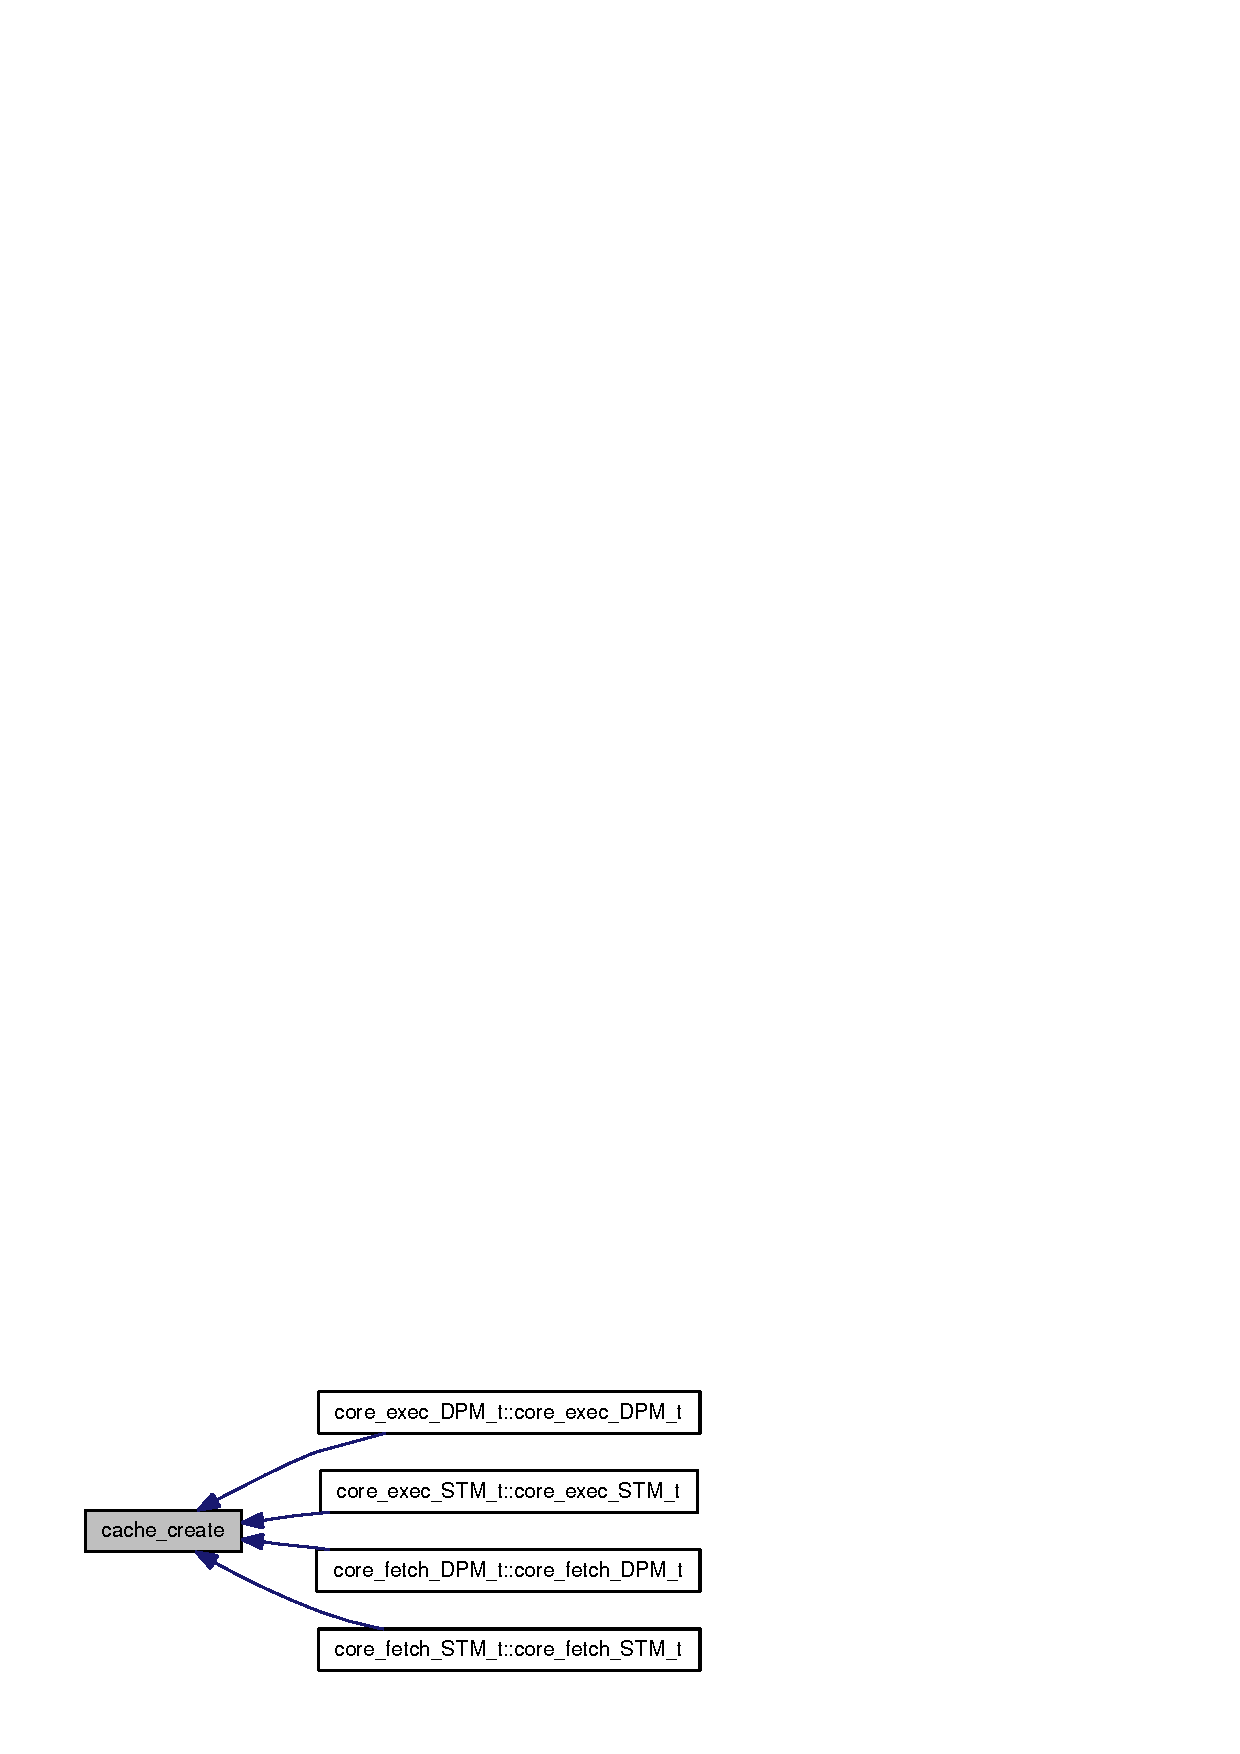
\includegraphics[width=170pt]{config_2zesto-cache_8cpp_76fc9319bafb600695d818375fe21ea3_icgraph}
\end{center}
\end{figure}
\index{config/zesto-cache.cpp@{config/zesto-cache.cpp}!cache\_\-enqueuable@{cache\_\-enqueuable}}
\index{cache\_\-enqueuable@{cache\_\-enqueuable}!config/zesto-cache.cpp@{config/zesto-cache.cpp}}
\subsubsection[{cache\_\-enqueuable}]{\setlength{\rightskip}{0pt plus 5cm}int cache\_\-enqueuable (const struct {\bf cache\_\-t} $\ast$const  {\em cp}, \/  const int {\em thread\_\-id}, \/  const {\bf md\_\-paddr\_\-t} {\em addr})}\label{config_2zesto-cache_8cpp_35c7c82c117f5713ec55d40f831060da}




Definition at line 1076 of file config/zesto-cache.cpp.

Referenced by cache\_\-prefetch(), cache\_\-prefetch\_\-llc(), cache\_\-process(), core\_\-exec\_\-STM\_\-t::LDQ\_\-schedule(), core\_\-exec\_\-DPM\_\-t::LDQ\_\-schedule(), core\_\-fetch\_\-STM\_\-t::step(), core\_\-fetch\_\-DPM\_\-t::step(), core\_\-exec\_\-STM\_\-t::STQ\_\-deallocate\_\-std(), and core\_\-exec\_\-DPM\_\-t::STQ\_\-deallocate\_\-std().

Here is the caller graph for this function:\nopagebreak
\begin{figure}[H]
\begin{center}
\leavevmode
\includegraphics[width=420pt]{config_2zesto-cache_8cpp_35c7c82c117f5713ec55d40f831060da_icgraph}
\end{center}
\end{figure}
\index{config/zesto-cache.cpp@{config/zesto-cache.cpp}!cache\_\-enqueue@{cache\_\-enqueue}}
\index{cache\_\-enqueue@{cache\_\-enqueue}!config/zesto-cache.cpp@{config/zesto-cache.cpp}}
\subsubsection[{cache\_\-enqueue}]{\setlength{\rightskip}{0pt plus 5cm}void cache\_\-enqueue (struct {\bf core\_\-t} $\ast$const  {\em core}, \/  struct {\bf cache\_\-t} $\ast$const  {\em cp}, \/  struct {\bf cache\_\-t} $\ast$const  {\em prev\_\-cp}, \/  const enum {\bf cache\_\-command} {\em cmd}, \/  const int {\em thread\_\-id}, \/  const {\bf md\_\-addr\_\-t} {\em PC}, \/  const {\bf md\_\-paddr\_\-t} {\em addr}, \/  const {\bf seq\_\-t} {\em action\_\-id}, \/  const int {\em MSHR\_\-bank}, \/  const int {\em MSHR\_\-index}, \/  void $\ast$const  {\em op}, \/  void($\ast$)(void $\ast$) {\em cb}, \/  void($\ast$)(void $\ast$, int) {\em miss\_\-cb}, \/  bool($\ast$)(void $\ast$, {\bf seq\_\-t}) {\em translated\_\-cb}, \/  {\bf seq\_\-t}($\ast$)(void $\ast$) {\em get\_\-action\_\-id})}\label{config_2zesto-cache_8cpp_0831369c0f015a2e350b71f2fc445c70}




Definition at line 1095 of file config/zesto-cache.cpp.

Referenced by cache\_\-prefetch(), cache\_\-prefetch\_\-llc(), cache\_\-process(), core\_\-exec\_\-STM\_\-t::LDQ\_\-schedule(), core\_\-exec\_\-DPM\_\-t::LDQ\_\-schedule(), core\_\-fetch\_\-STM\_\-t::step(), core\_\-fetch\_\-DPM\_\-t::step(), core\_\-exec\_\-STM\_\-t::STQ\_\-deallocate\_\-std(), and core\_\-exec\_\-DPM\_\-t::STQ\_\-deallocate\_\-std().

Here is the caller graph for this function:\nopagebreak
\begin{figure}[H]
\begin{center}
\leavevmode
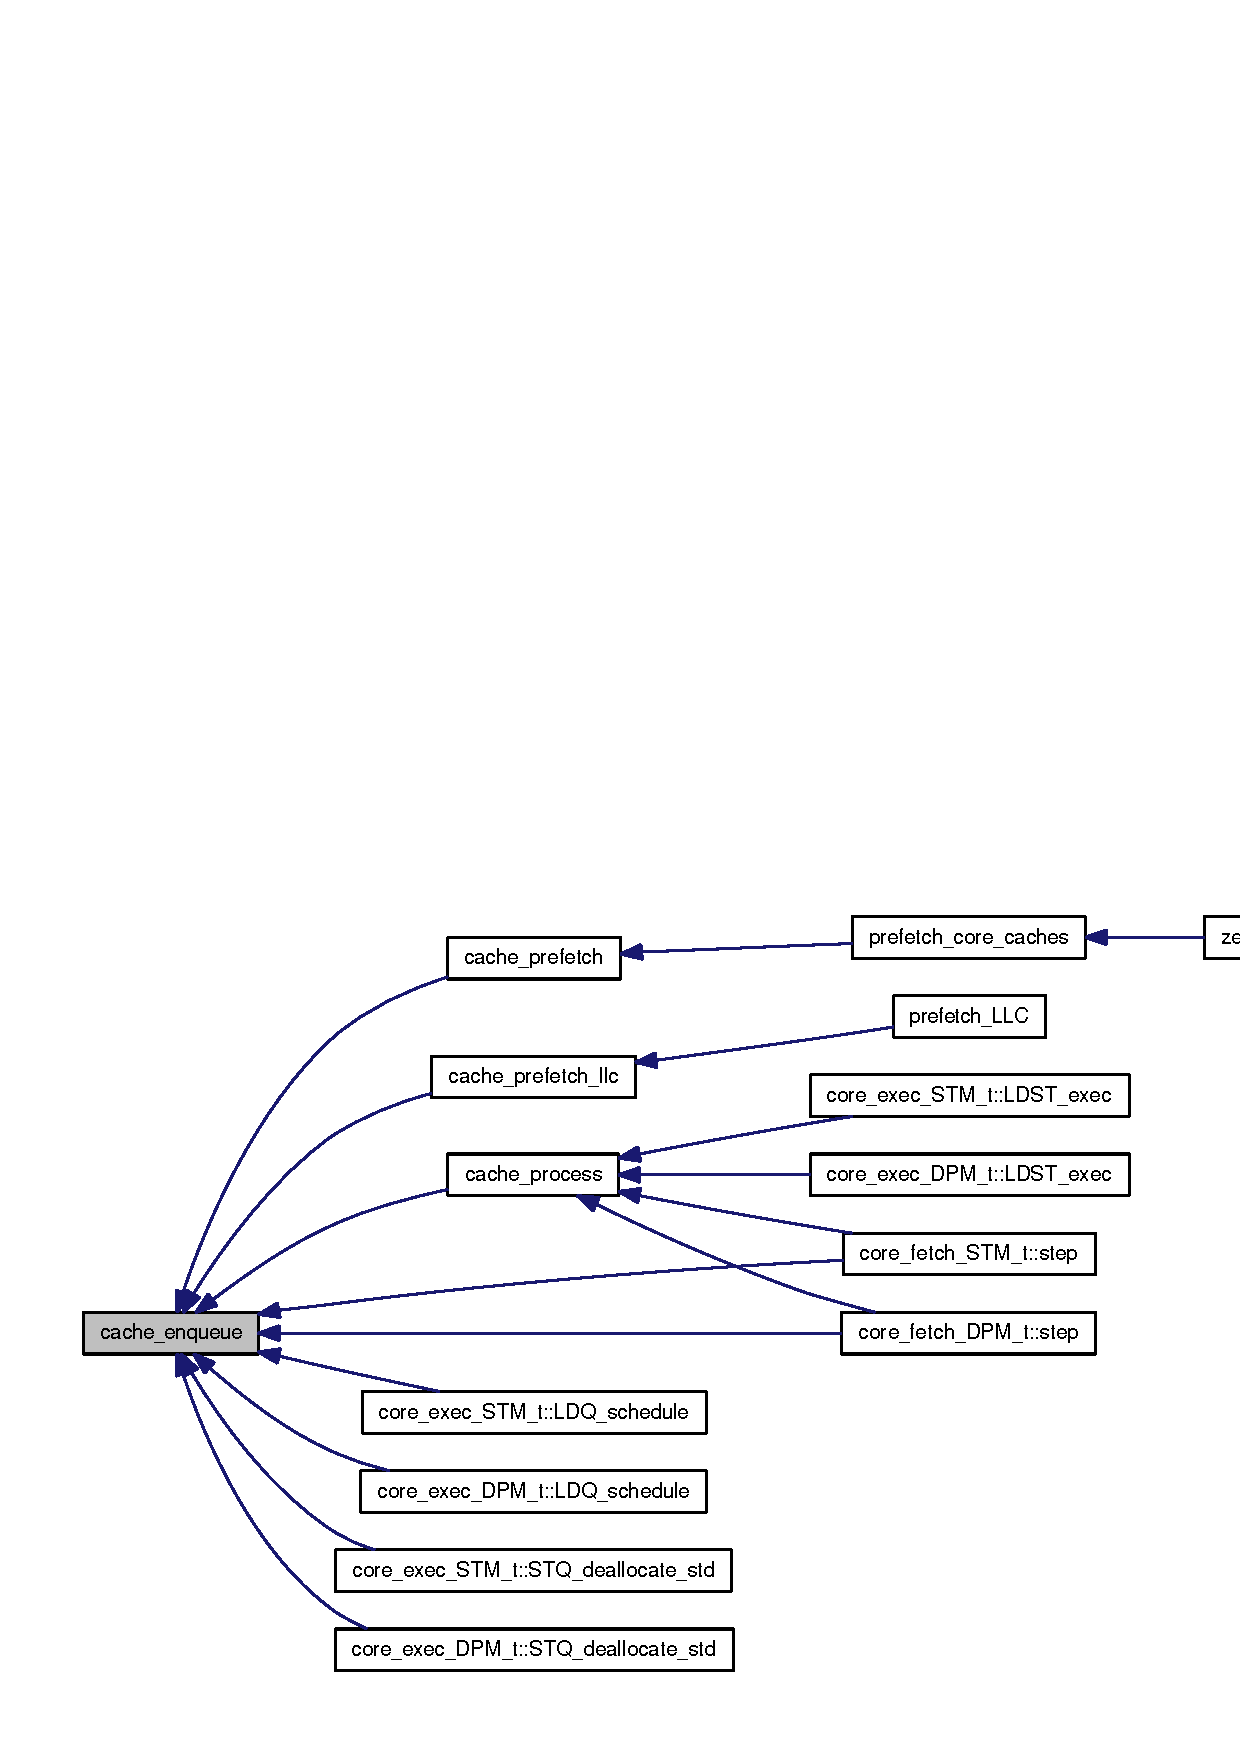
\includegraphics[width=420pt]{config_2zesto-cache_8cpp_0831369c0f015a2e350b71f2fc445c70_icgraph}
\end{center}
\end{figure}
\index{config/zesto-cache.cpp@{config/zesto-cache.cpp}!cache\_\-fill@{cache\_\-fill}}
\index{cache\_\-fill@{cache\_\-fill}!config/zesto-cache.cpp@{config/zesto-cache.cpp}}
\subsubsection[{cache\_\-fill}]{\setlength{\rightskip}{0pt plus 5cm}static void cache\_\-fill (struct {\bf cache\_\-t} $\ast$const  {\em cp}, \/  const enum {\bf cache\_\-command} {\em cmd}, \/  const {\bf md\_\-paddr\_\-t} {\em paddr}, \/  struct {\bf core\_\-t} $\ast$ {\em core})\hspace{0.3cm}{\tt  [inline, static]}}\label{config_2zesto-cache_8cpp_4268c8076eb193fe97abe55263b81c9c}




Definition at line 1486 of file config/zesto-cache.cpp.

References cache\_\-assert, cache\_\-t::check\_\-for\_\-fill\_\-work, cache\_\-t::check\_\-for\_\-work, cache\_\-fill\_\-t::cmd, cache\_\-fill\_\-t::core, fill\_\-heap\_\-balance(), cache\_\-t::fill\_\-num, cache\_\-t::fill\_\-pipe, GET\_\-BANK, cache\_\-t::latency, cache\_\-fill\_\-t::paddr, cache\_\-fill\_\-t::pipe\_\-exit\_\-time, sim\_\-cycle, and cache\_\-fill\_\-t::valid.

Referenced by cache\_\-process().

Here is the caller graph for this function:\nopagebreak
\begin{figure}[H]
\begin{center}
\leavevmode
\includegraphics[width=205pt]{config_2zesto-cache_8cpp_4268c8076eb193fe97abe55263b81c9c_icgraph}
\end{center}
\end{figure}
\index{config/zesto-cache.cpp@{config/zesto-cache.cpp}!cache\_\-fillable@{cache\_\-fillable}}
\index{cache\_\-fillable@{cache\_\-fillable}!config/zesto-cache.cpp@{config/zesto-cache.cpp}}
\subsubsection[{cache\_\-fillable}]{\setlength{\rightskip}{0pt plus 5cm}static bool cache\_\-fillable (const struct {\bf cache\_\-t} $\ast$const  {\em cp}, \/  const {\bf md\_\-paddr\_\-t} {\em paddr})\hspace{0.3cm}{\tt  [inline, static]}}\label{config_2zesto-cache_8cpp_b1883760de25022c2b30d602d5b50c4a}




Definition at line 1474 of file config/zesto-cache.cpp.

References cache\_\-t::fill\_\-num, GET\_\-BANK, and cache\_\-t::latency.

Referenced by cache\_\-process().

Here is the caller graph for this function:\nopagebreak
\begin{figure}[H]
\begin{center}
\leavevmode
\includegraphics[width=214pt]{config_2zesto-cache_8cpp_b1883760de25022c2b30d602d5b50c4a_icgraph}
\end{center}
\end{figure}
\index{config/zesto-cache.cpp@{config/zesto-cache.cpp}!cache\_\-freeze\_\-stats@{cache\_\-freeze\_\-stats}}
\index{cache\_\-freeze\_\-stats@{cache\_\-freeze\_\-stats}!config/zesto-cache.cpp@{config/zesto-cache.cpp}}
\subsubsection[{cache\_\-freeze\_\-stats}]{\setlength{\rightskip}{0pt plus 5cm}void cache\_\-freeze\_\-stats (struct {\bf core\_\-t} $\ast$const  {\em core})}\label{config_2zesto-cache_8cpp_bd1fe8334f2259dc773b85f98c7fbcfa}




Definition at line 2402 of file config/zesto-cache.cpp.

Referenced by core\_\-commit\_\-STM\_\-t::step(), and core\_\-commit\_\-DPM\_\-t::step().

Here is the caller graph for this function:\nopagebreak
\begin{figure}[H]
\begin{center}
\leavevmode
\includegraphics[width=157pt]{config_2zesto-cache_8cpp_bd1fe8334f2259dc773b85f98c7fbcfa_icgraph}
\end{center}
\end{figure}
\index{config/zesto-cache.cpp@{config/zesto-cache.cpp}!cache\_\-get\_\-evictee@{cache\_\-get\_\-evictee}}
\index{cache\_\-get\_\-evictee@{cache\_\-get\_\-evictee}!config/zesto-cache.cpp@{config/zesto-cache.cpp}}
\subsubsection[{cache\_\-get\_\-evictee}]{\setlength{\rightskip}{0pt plus 5cm}struct {\bf cache\_\-line\_\-t}$\ast$ cache\_\-get\_\-evictee (struct {\bf cache\_\-t} $\ast$const  {\em cp}, \/  const {\bf md\_\-paddr\_\-t} {\em addr}, \/  {\bf core\_\-t} $\ast$const  {\em core})\hspace{0.3cm}{\tt  [read]}}\label{config_2zesto-cache_8cpp_64ef5d6d0aef624c6534b1aae0416f96}




Definition at line 840 of file config/zesto-cache.cpp.

Referenced by cache\_\-process(), and sim\_\-fastfwd().

Here is the caller graph for this function:\nopagebreak
\begin{figure}[H]
\begin{center}
\leavevmode
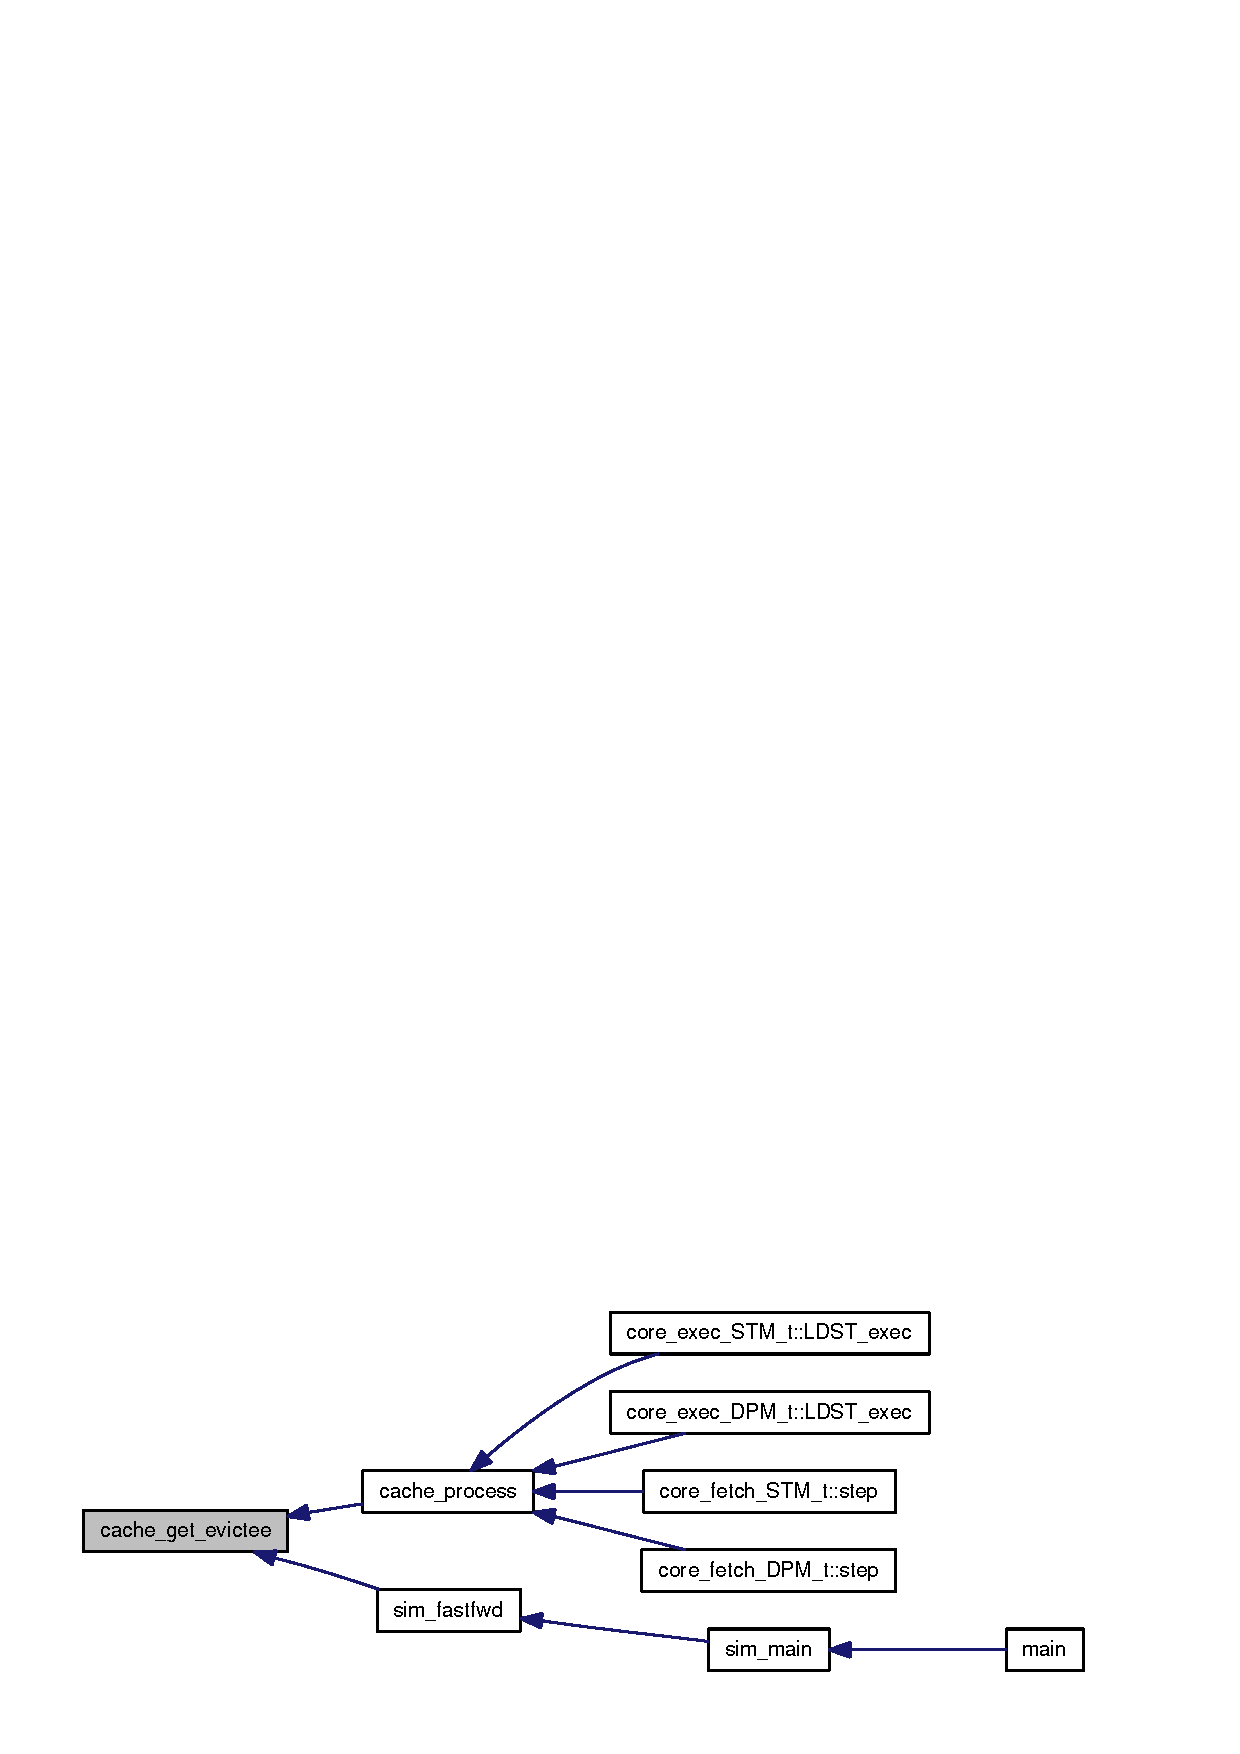
\includegraphics[width=262pt]{config_2zesto-cache_8cpp_64ef5d6d0aef624c6534b1aae0416f96_icgraph}
\end{center}
\end{figure}
\index{config/zesto-cache.cpp@{config/zesto-cache.cpp}!cache\_\-heap\_\-balance@{cache\_\-heap\_\-balance}}
\index{cache\_\-heap\_\-balance@{cache\_\-heap\_\-balance}!config/zesto-cache.cpp@{config/zesto-cache.cpp}}
\subsubsection[{cache\_\-heap\_\-balance}]{\setlength{\rightskip}{0pt plus 5cm}static void cache\_\-heap\_\-balance (struct {\bf cache\_\-action\_\-t} $\ast$const  {\em pipe}, \/  const int {\em insert\_\-position})\hspace{0.3cm}{\tt  [static]}}\label{config_2zesto-cache_8cpp_0784d914ca0e1dc0f651a456830f94ed}




Definition at line 981 of file config/zesto-cache.cpp.

References memswap().

Referenced by cache\_\-enqueue(), and cache\_\-enqueue\_\-llc().

Here is the caller graph for this function:\nopagebreak
\begin{figure}[H]
\begin{center}
\leavevmode
\includegraphics[width=420pt]{config_2zesto-cache_8cpp_0784d914ca0e1dc0f651a456830f94ed_icgraph}
\end{center}
\end{figure}
\index{config/zesto-cache.cpp@{config/zesto-cache.cpp}!cache\_\-heap\_\-remove@{cache\_\-heap\_\-remove}}
\index{cache\_\-heap\_\-remove@{cache\_\-heap\_\-remove}!config/zesto-cache.cpp@{config/zesto-cache.cpp}}
\subsubsection[{cache\_\-heap\_\-remove}]{\setlength{\rightskip}{0pt plus 5cm}static void cache\_\-heap\_\-remove (struct {\bf cache\_\-action\_\-t} $\ast$const  {\em pipe}, \/  const int {\em pipe\_\-num})\hspace{0.3cm}{\tt  [static]}}\label{config_2zesto-cache_8cpp_672e06f81a893ac6af2c4fd4948069ed}




Definition at line 1007 of file config/zesto-cache.cpp.

References cache\_\-action\_\-t::cb, memswap(), cache\_\-action\_\-t::pipe\_\-exit\_\-time, and TICK\_\-T\_\-MAX.

Referenced by cache\_\-process(), and cache\_\-process\_\-llc().

Here is the caller graph for this function:\nopagebreak
\begin{figure}[H]
\begin{center}
\leavevmode
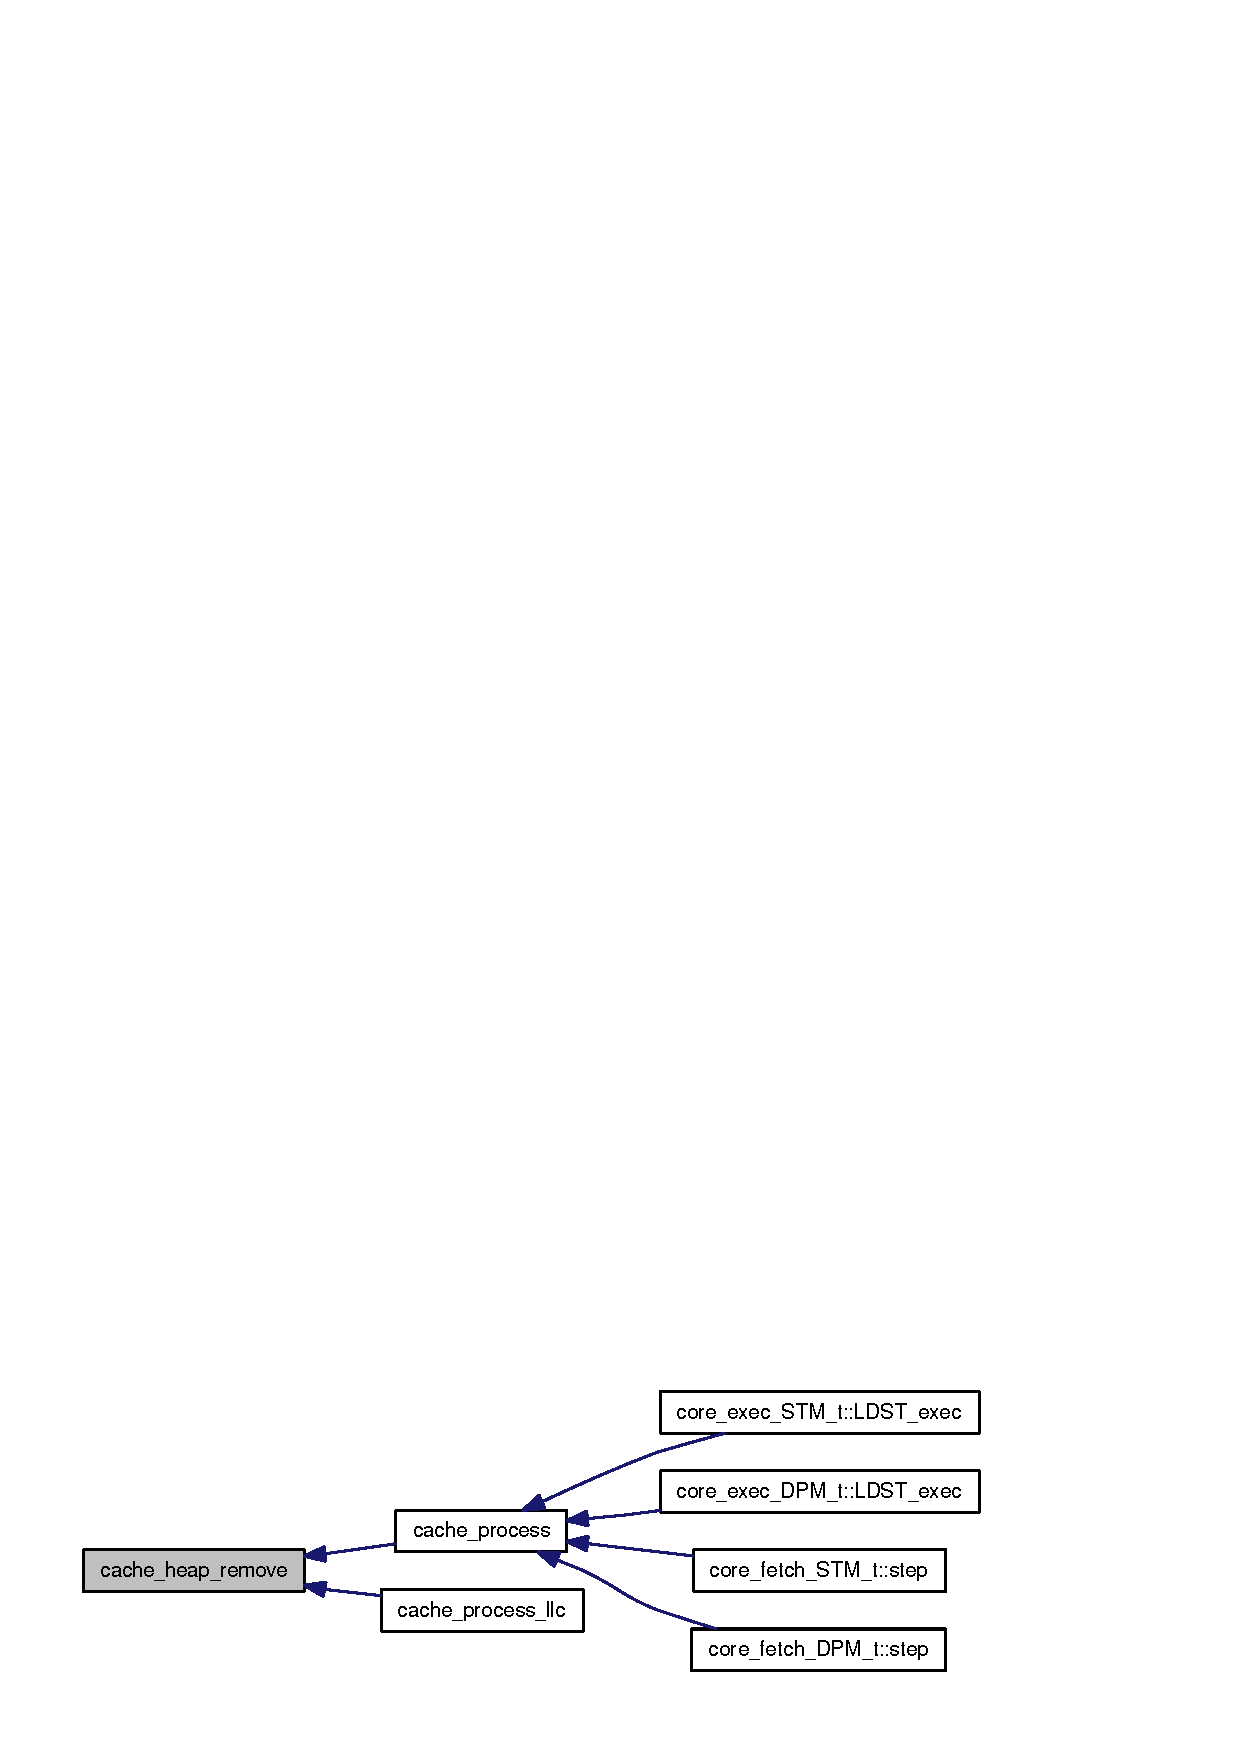
\includegraphics[width=237pt]{config_2zesto-cache_8cpp_672e06f81a893ac6af2c4fd4948069ed_icgraph}
\end{center}
\end{figure}
\index{config/zesto-cache.cpp@{config/zesto-cache.cpp}!cache\_\-insert\_\-block@{cache\_\-insert\_\-block}}
\index{cache\_\-insert\_\-block@{cache\_\-insert\_\-block}!config/zesto-cache.cpp@{config/zesto-cache.cpp}}
\subsubsection[{cache\_\-insert\_\-block}]{\setlength{\rightskip}{0pt plus 5cm}void cache\_\-insert\_\-block (struct {\bf cache\_\-t} $\ast$const  {\em cp}, \/  const enum {\bf cache\_\-command} {\em cmd}, \/  const {\bf md\_\-paddr\_\-t} {\em addr}, \/  {\bf core\_\-t} $\ast$const  {\em core})}\label{config_2zesto-cache_8cpp_1f7522c0547a72f15e199abba2f63812}




Definition at line 742 of file config/zesto-cache.cpp.

Referenced by cache\_\-process(), and sim\_\-fastfwd().

Here is the caller graph for this function:\nopagebreak
\begin{figure}[H]
\begin{center}
\leavevmode
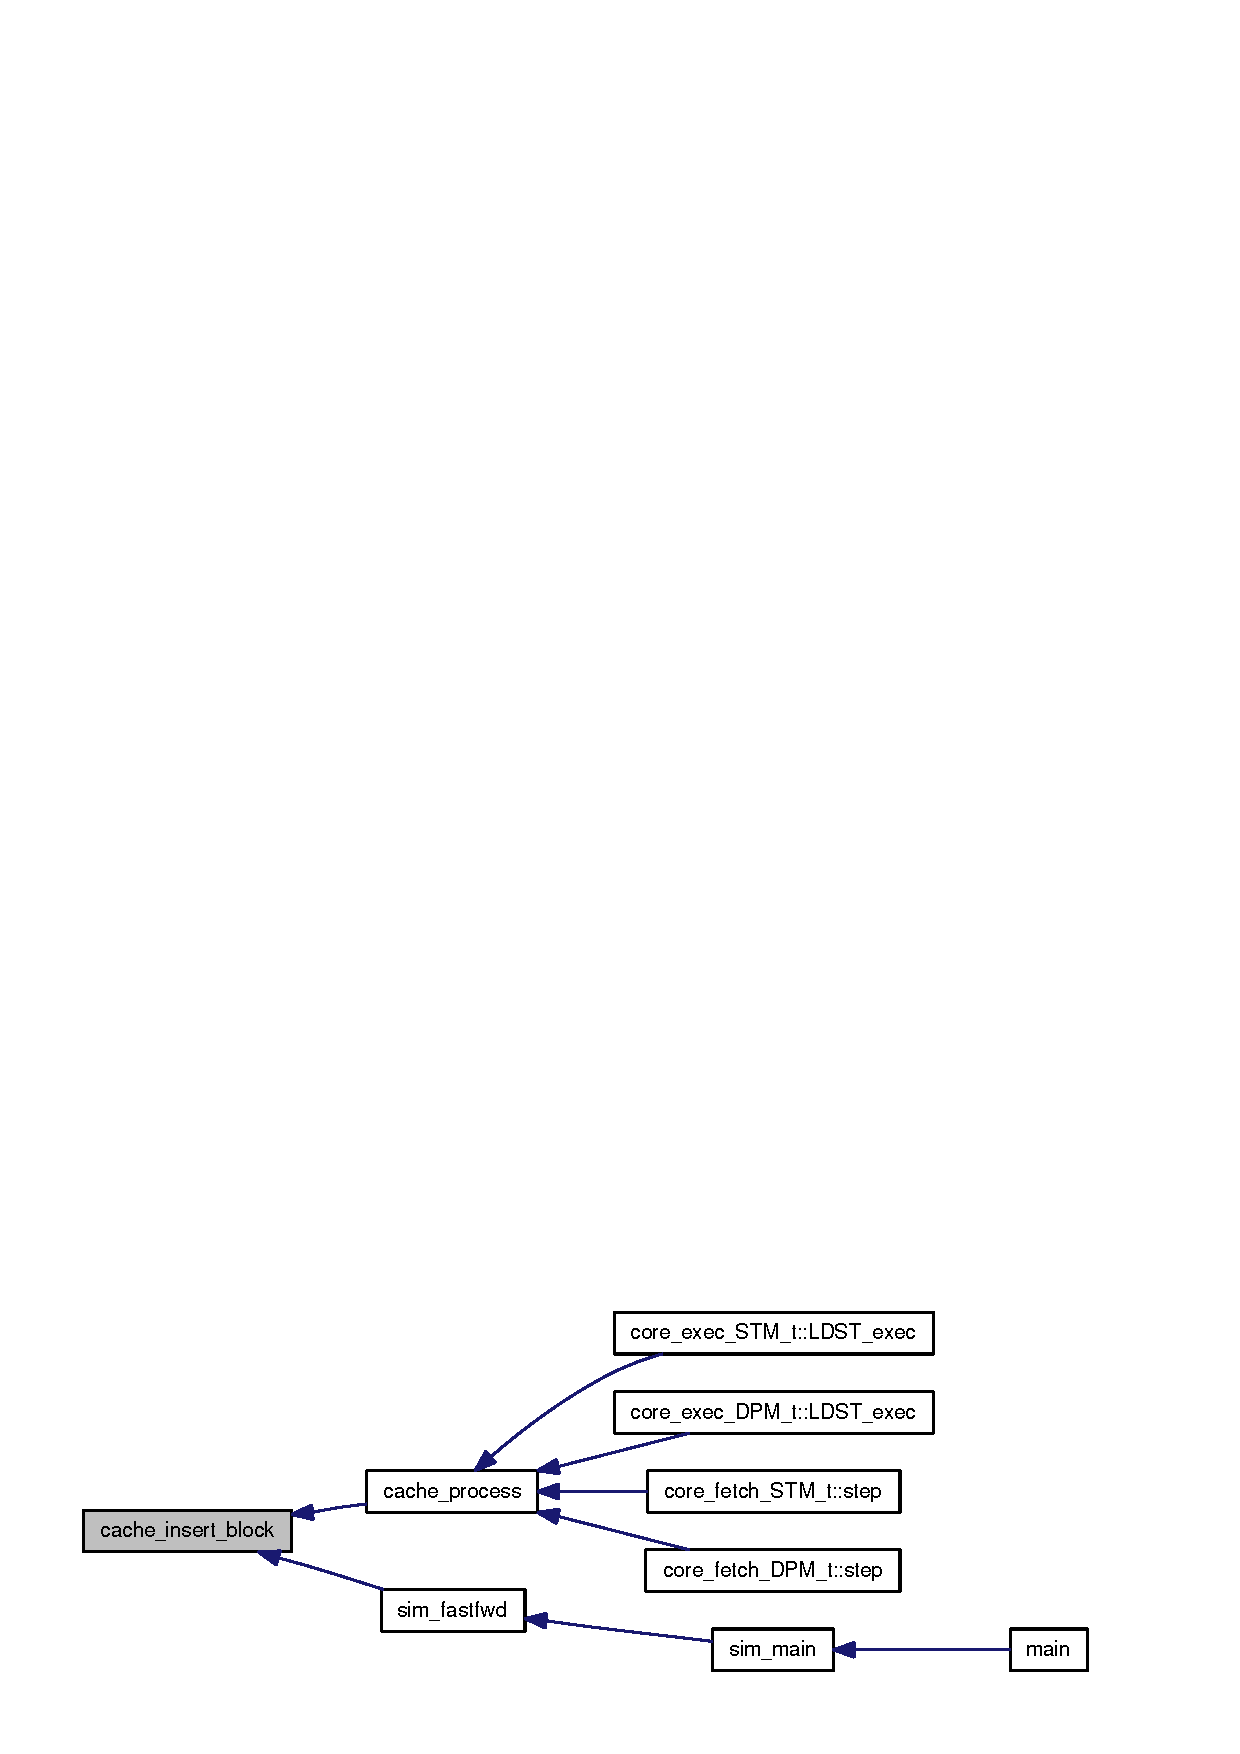
\includegraphics[width=263pt]{config_2zesto-cache_8cpp_1f7522c0547a72f15e199abba2f63812_icgraph}
\end{center}
\end{figure}
\index{config/zesto-cache.cpp@{config/zesto-cache.cpp}!cache\_\-is\_\-hit@{cache\_\-is\_\-hit}}
\index{cache\_\-is\_\-hit@{cache\_\-is\_\-hit}!config/zesto-cache.cpp@{config/zesto-cache.cpp}}
\subsubsection[{cache\_\-is\_\-hit}]{\setlength{\rightskip}{0pt plus 5cm}struct {\bf cache\_\-line\_\-t}$\ast$ cache\_\-is\_\-hit (struct {\bf cache\_\-t} $\ast$const  {\em cp}, \/  const enum {\bf cache\_\-command} {\em cmd}, \/  const {\bf md\_\-paddr\_\-t} {\em addr}, \/  struct {\bf core\_\-t} $\ast$const  {\em core})\hspace{0.3cm}{\tt  [read]}}\label{config_2zesto-cache_8cpp_bbba2e5ba6186173122bcf1e35dc56eb}




Definition at line 618 of file config/zesto-cache.cpp.

Referenced by cache\_\-process(), and sim\_\-fastfwd().

Here is the caller graph for this function:\nopagebreak
\begin{figure}[H]
\begin{center}
\leavevmode
\includegraphics[width=249pt]{config_2zesto-cache_8cpp_bbba2e5ba6186173122bcf1e35dc56eb_icgraph}
\end{center}
\end{figure}
\index{config/zesto-cache.cpp@{config/zesto-cache.cpp}!cache\_\-peek@{cache\_\-peek}}
\index{cache\_\-peek@{cache\_\-peek}!config/zesto-cache.cpp@{config/zesto-cache.cpp}}
\subsubsection[{cache\_\-peek}]{\setlength{\rightskip}{0pt plus 5cm}static struct {\bf cache\_\-line\_\-t}$\ast$ cache\_\-peek (const struct {\bf cache\_\-t} $\ast$const  {\em cp}, \/  const {\bf md\_\-paddr\_\-t} {\em addr})\hspace{0.3cm}{\tt  [static, read]}}\label{config_2zesto-cache_8cpp_32083cc0a79d18fbb1932fca2d15df1e}




Definition at line 717 of file config/zesto-cache.cpp.

References cache\_\-t::addr\_\-shift, cache\_\-t::blocks, cache\_\-line\_\-t::next, cache\_\-t::sets, cache\_\-line\_\-t::tag, and cache\_\-line\_\-t::valid.

Referenced by cache\_\-invalidate(), and cache\_\-process().

Here is the caller graph for this function:\nopagebreak
\begin{figure}[H]
\begin{center}
\leavevmode
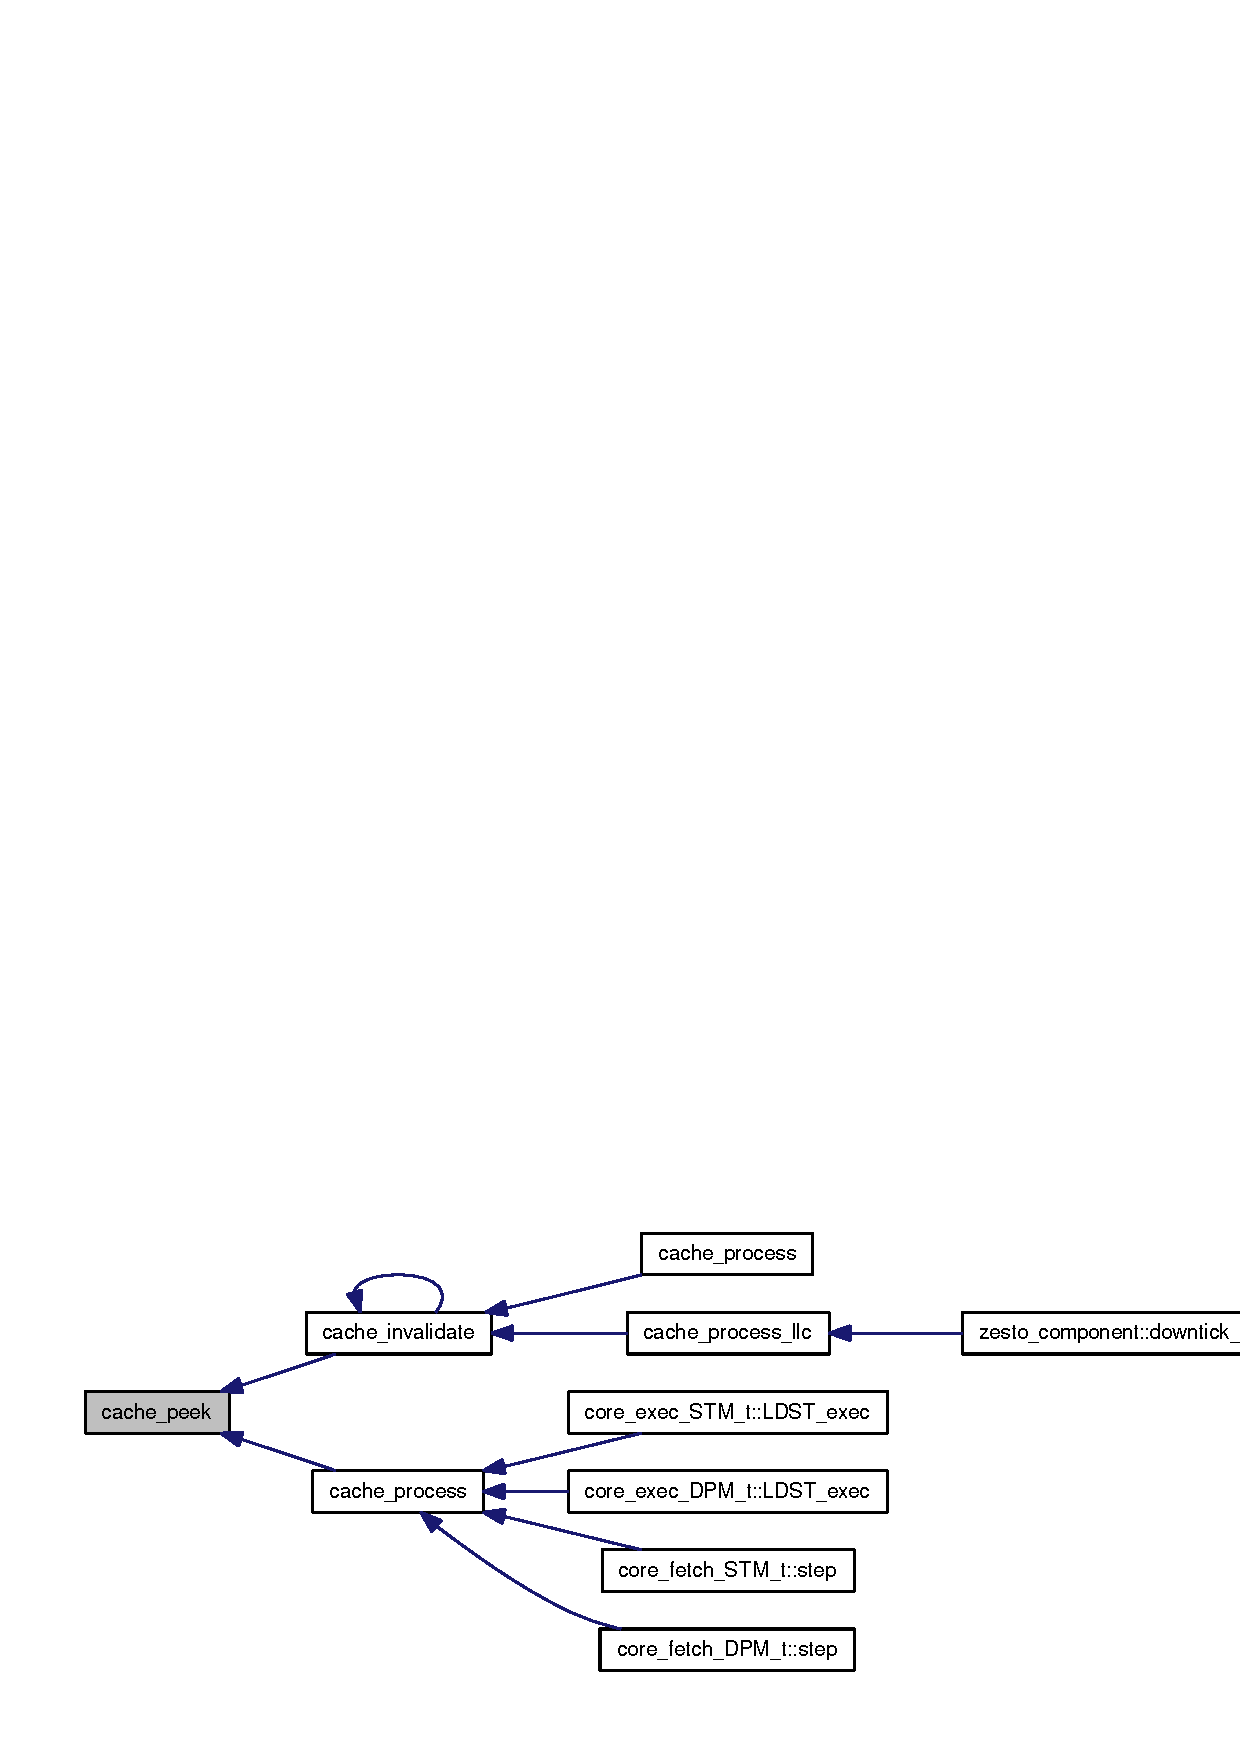
\includegraphics[width=420pt]{config_2zesto-cache_8cpp_32083cc0a79d18fbb1932fca2d15df1e_icgraph}
\end{center}
\end{figure}
\index{config/zesto-cache.cpp@{config/zesto-cache.cpp}!cache\_\-prefetch@{cache\_\-prefetch}}
\index{cache\_\-prefetch@{cache\_\-prefetch}!config/zesto-cache.cpp@{config/zesto-cache.cpp}}
\subsubsection[{cache\_\-prefetch}]{\setlength{\rightskip}{0pt plus 5cm}static void cache\_\-prefetch (struct {\bf cache\_\-t} $\ast$const  {\em cp})\hspace{0.3cm}{\tt  [static]}}\label{config_2zesto-cache_8cpp_488a1ffa67f67839ee35d6925c2162d8}




Definition at line 2343 of file config/zesto-cache.cpp.

References cache\_\-t::cache\_\-t::PFF\_\-t::addr, cache\_\-assert, cache\_\-enqueuable(), cache\_\-enqueue(), CACHE\_\-PREFETCH, cache\_\-t::cache\_\-t::PFF\_\-t::core, DO\_\-NOT\_\-TRANSLATE, dummy\_\-callback(), GET\_\-MSHR\_\-BANK, modinc(), NO\_\-MSHR, cache\_\-t::cache\_\-t::PFF\_\-t::PC, PF\_\-OK, cache\_\-t::PF\_\-sample\_\-interval, cache\_\-t::PF\_\-state, cache\_\-t::PFF, cache\_\-t::PFF\_\-head, cache\_\-t::PFF\_\-num, cache\_\-t::PFF\_\-size, cache\_\-t::prefetch\_\-max, and cache\_\-t::prefetch\_\-threshold.

Referenced by prefetch\_\-core\_\-caches().

Here is the caller graph for this function:\nopagebreak
\begin{figure}[H]
\begin{center}
\leavevmode
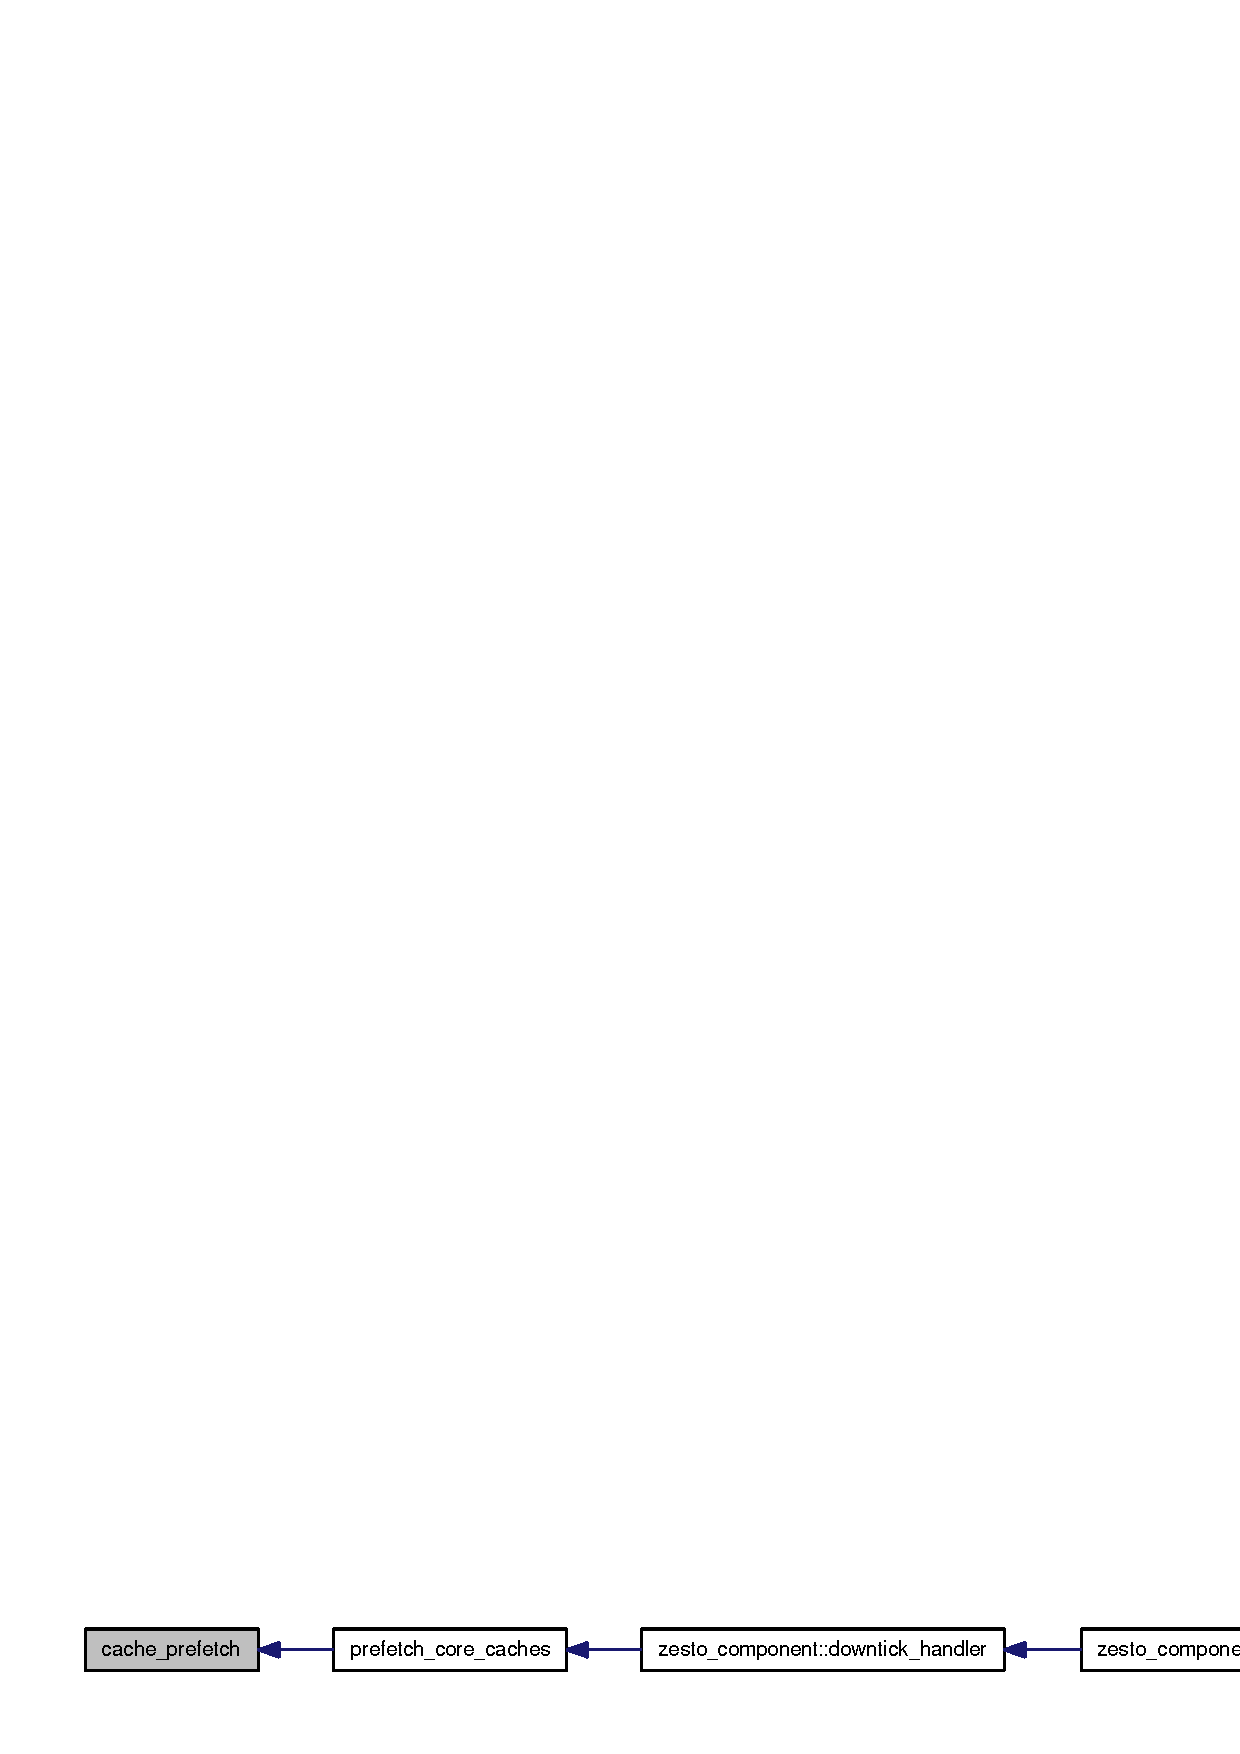
\includegraphics[width=387pt]{config_2zesto-cache_8cpp_488a1ffa67f67839ee35d6925c2162d8_icgraph}
\end{center}
\end{figure}
\index{config/zesto-cache.cpp@{config/zesto-cache.cpp}!cache\_\-print@{cache\_\-print}}
\index{cache\_\-print@{cache\_\-print}!config/zesto-cache.cpp@{config/zesto-cache.cpp}}
\subsubsection[{cache\_\-print}]{\setlength{\rightskip}{0pt plus 5cm}void cache\_\-print (const struct {\bf cache\_\-t} $\ast$const  {\em cp})}\label{config_2zesto-cache_8cpp_5e18254876909dd853b5bdd65556188f}




Definition at line 2412 of file config/zesto-cache.cpp.

References cache\_\-t::banks, CACHE\_\-READ, CACHE\_\-WRITE, CACHE\_\-WRITEBACK, cache\_\-action\_\-t::cb, cache\_\-action\_\-t::cmd, cache\_\-t::fill\_\-pipe, cache\_\-t::latency, cache\_\-t::MSHR, cache\_\-t::MSHR\_\-size, cache\_\-t::name, cache\_\-action\_\-t::op, cache\_\-fill\_\-t::paddr, cache\_\-t::pipe, and cache\_\-fill\_\-t::valid.\index{config/zesto-cache.cpp@{config/zesto-cache.cpp}!cache\_\-process@{cache\_\-process}}
\index{cache\_\-process@{cache\_\-process}!config/zesto-cache.cpp@{config/zesto-cache.cpp}}
\subsubsection[{cache\_\-process}]{\setlength{\rightskip}{0pt plus 5cm}void cache\_\-process (struct {\bf cache\_\-t} $\ast$const  {\em cp})}\label{config_2zesto-cache_8cpp_93ce14ef87e7565964216ea27d912147}




Definition at line 1523 of file config/zesto-cache.cpp.

Referenced by core\_\-exec\_\-STM\_\-t::LDST\_\-exec(), core\_\-exec\_\-DPM\_\-t::LDST\_\-exec(), core\_\-fetch\_\-STM\_\-t::step(), and core\_\-fetch\_\-DPM\_\-t::step().

Here is the caller graph for this function:\nopagebreak
\begin{figure}[H]
\begin{center}
\leavevmode
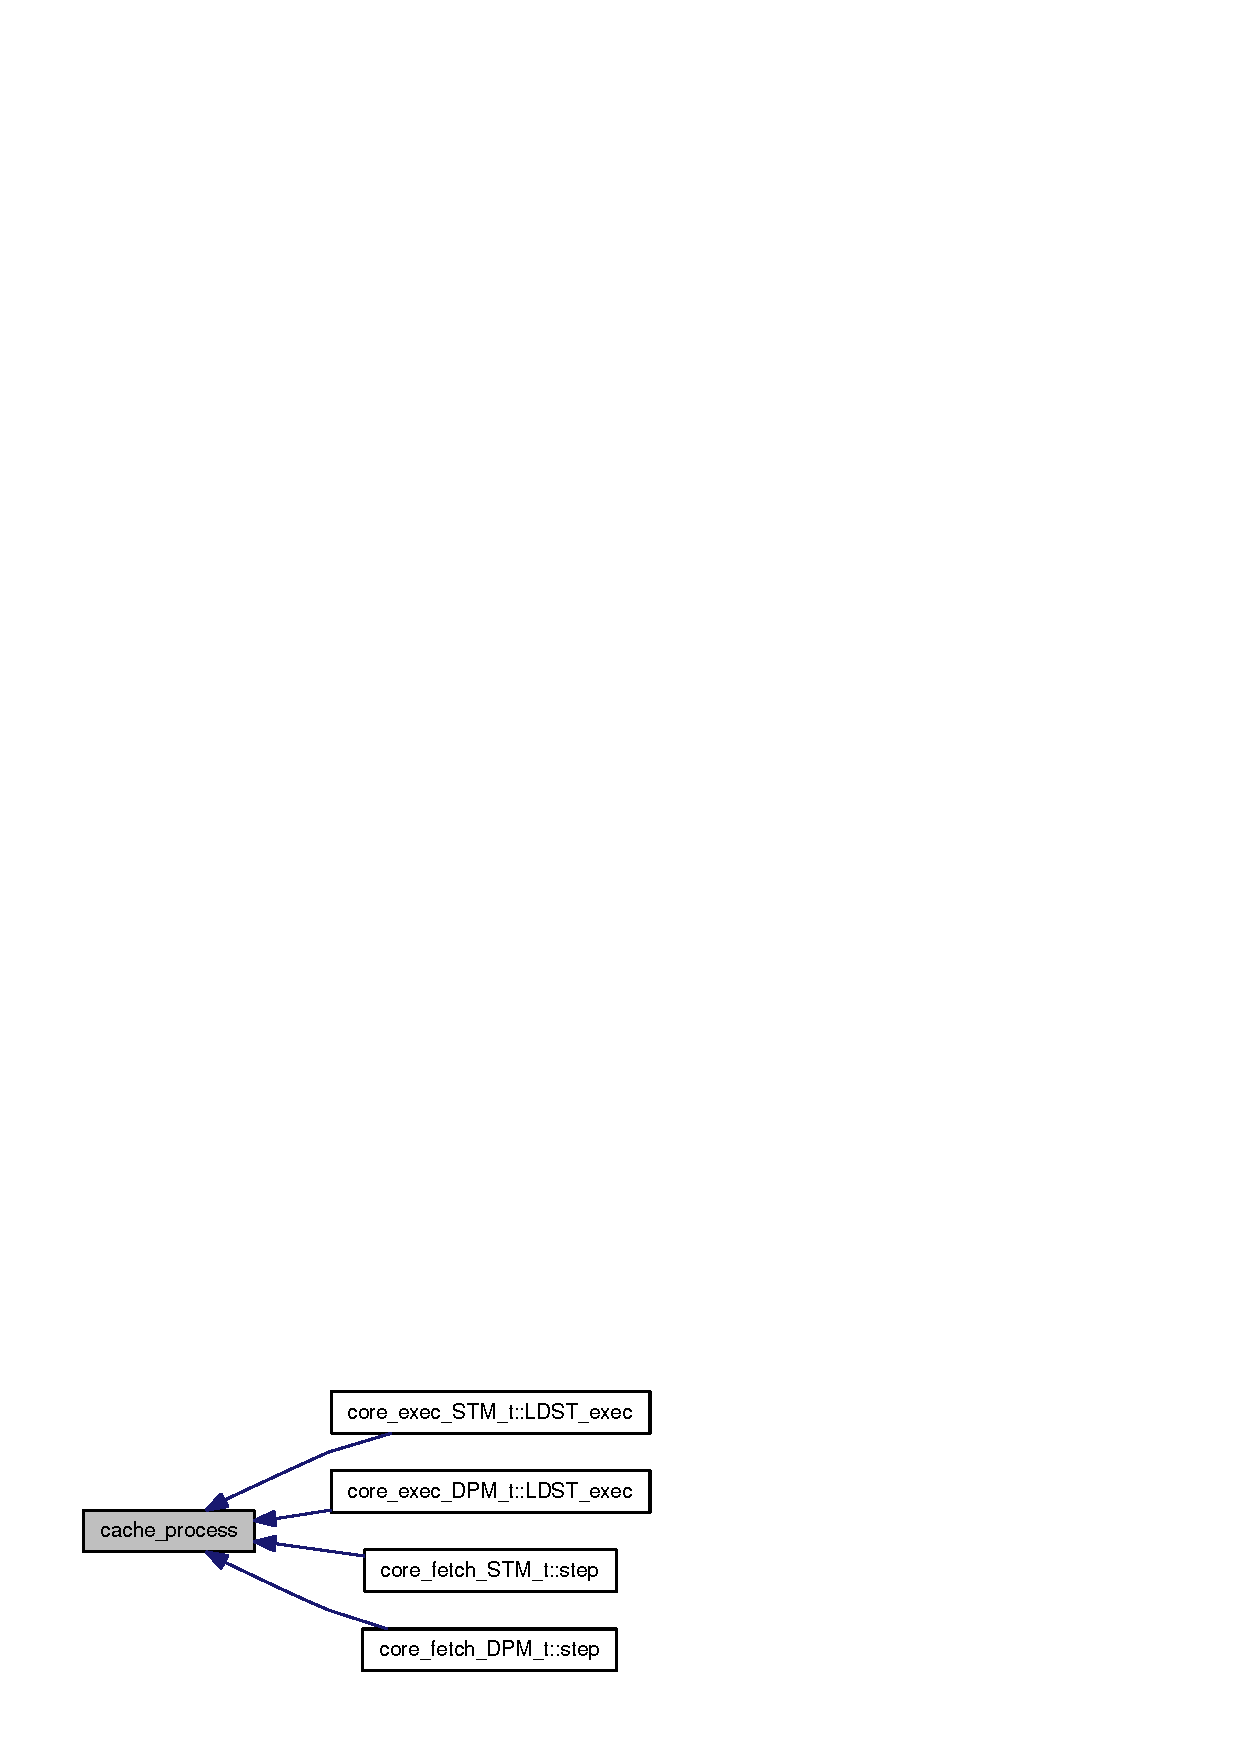
\includegraphics[width=158pt]{config_2zesto-cache_8cpp_93ce14ef87e7565964216ea27d912147_icgraph}
\end{center}
\end{figure}
\index{config/zesto-cache.cpp@{config/zesto-cache.cpp}!cache\_\-reg\_\-stats@{cache\_\-reg\_\-stats}}
\index{cache\_\-reg\_\-stats@{cache\_\-reg\_\-stats}!config/zesto-cache.cpp@{config/zesto-cache.cpp}}
\subsubsection[{cache\_\-reg\_\-stats}]{\setlength{\rightskip}{0pt plus 5cm}void cache\_\-reg\_\-stats (struct {\bf stat\_\-sdb\_\-t} $\ast$const  {\em sdb}, \/  const struct {\bf core\_\-t} $\ast$const  {\em core}, \/  struct {\bf cache\_\-t} $\ast$const  {\em cp})}\label{config_2zesto-cache_8cpp_80141f1bc8f06e0805162cdd6936c5d8}




Definition at line 280 of file config/zesto-cache.cpp.

Referenced by core\_\-fetch\_\-STM\_\-t::reg\_\-stats(), core\_\-fetch\_\-DPM\_\-t::reg\_\-stats(), core\_\-exec\_\-STM\_\-t::reg\_\-stats(), and core\_\-exec\_\-DPM\_\-t::reg\_\-stats().

Here is the caller graph for this function:\nopagebreak
\begin{figure}[H]
\begin{center}
\leavevmode
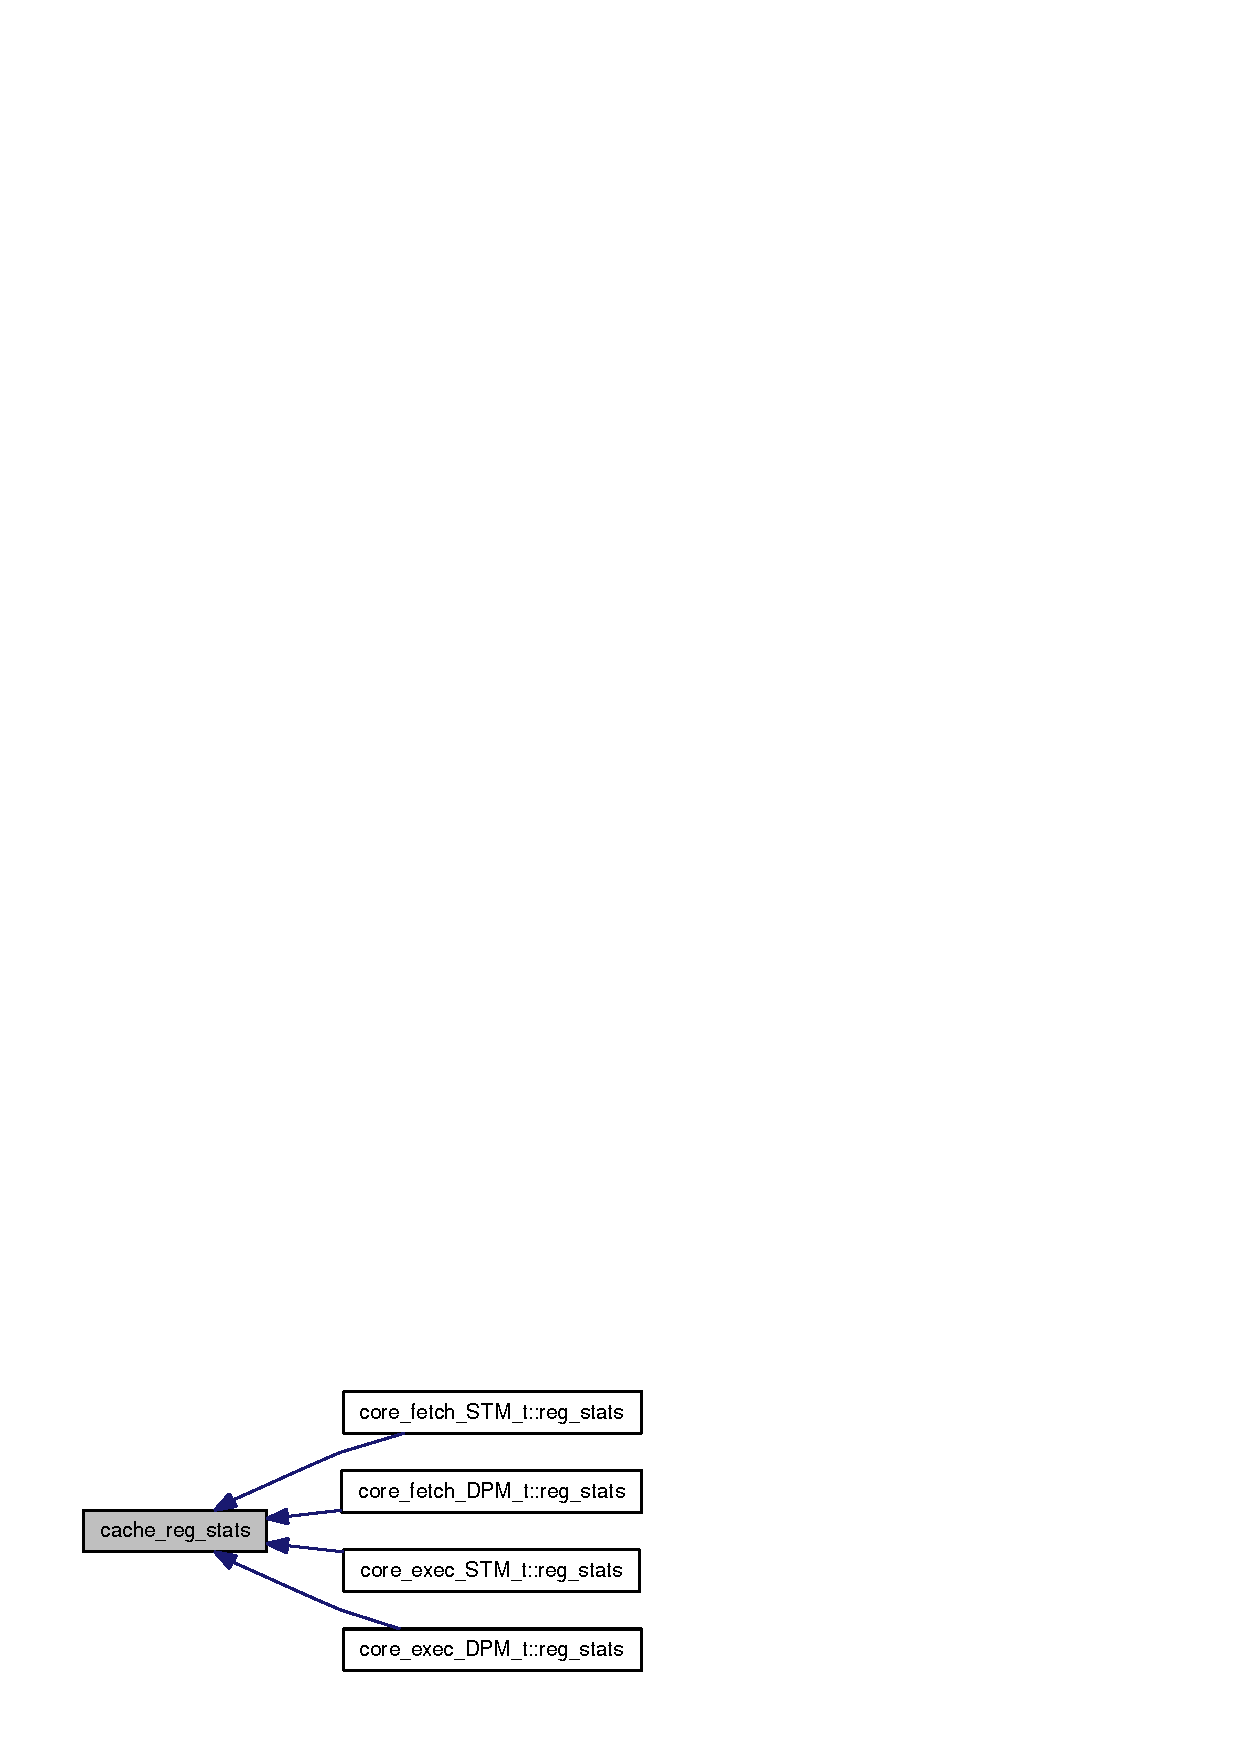
\includegraphics[width=156pt]{config_2zesto-cache_8cpp_80141f1bc8f06e0805162cdd6936c5d8_icgraph}
\end{center}
\end{figure}
\index{config/zesto-cache.cpp@{config/zesto-cache.cpp}!cache\_\-reset\_\-stats@{cache\_\-reset\_\-stats}}
\index{cache\_\-reset\_\-stats@{cache\_\-reset\_\-stats}!config/zesto-cache.cpp@{config/zesto-cache.cpp}}
\subsubsection[{cache\_\-reset\_\-stats}]{\setlength{\rightskip}{0pt plus 5cm}void cache\_\-reset\_\-stats (struct {\bf cache\_\-t} $\ast$const  {\em cp})}\label{config_2zesto-cache_8cpp_aff01697c94f19565dfd6d631bf4bf76}




Definition at line 515 of file config/zesto-cache.cpp.

Referenced by emergency\_\-recovery(), and sim\_\-fastfwd().

Here is the caller graph for this function:\nopagebreak
\begin{figure}[H]
\begin{center}
\leavevmode
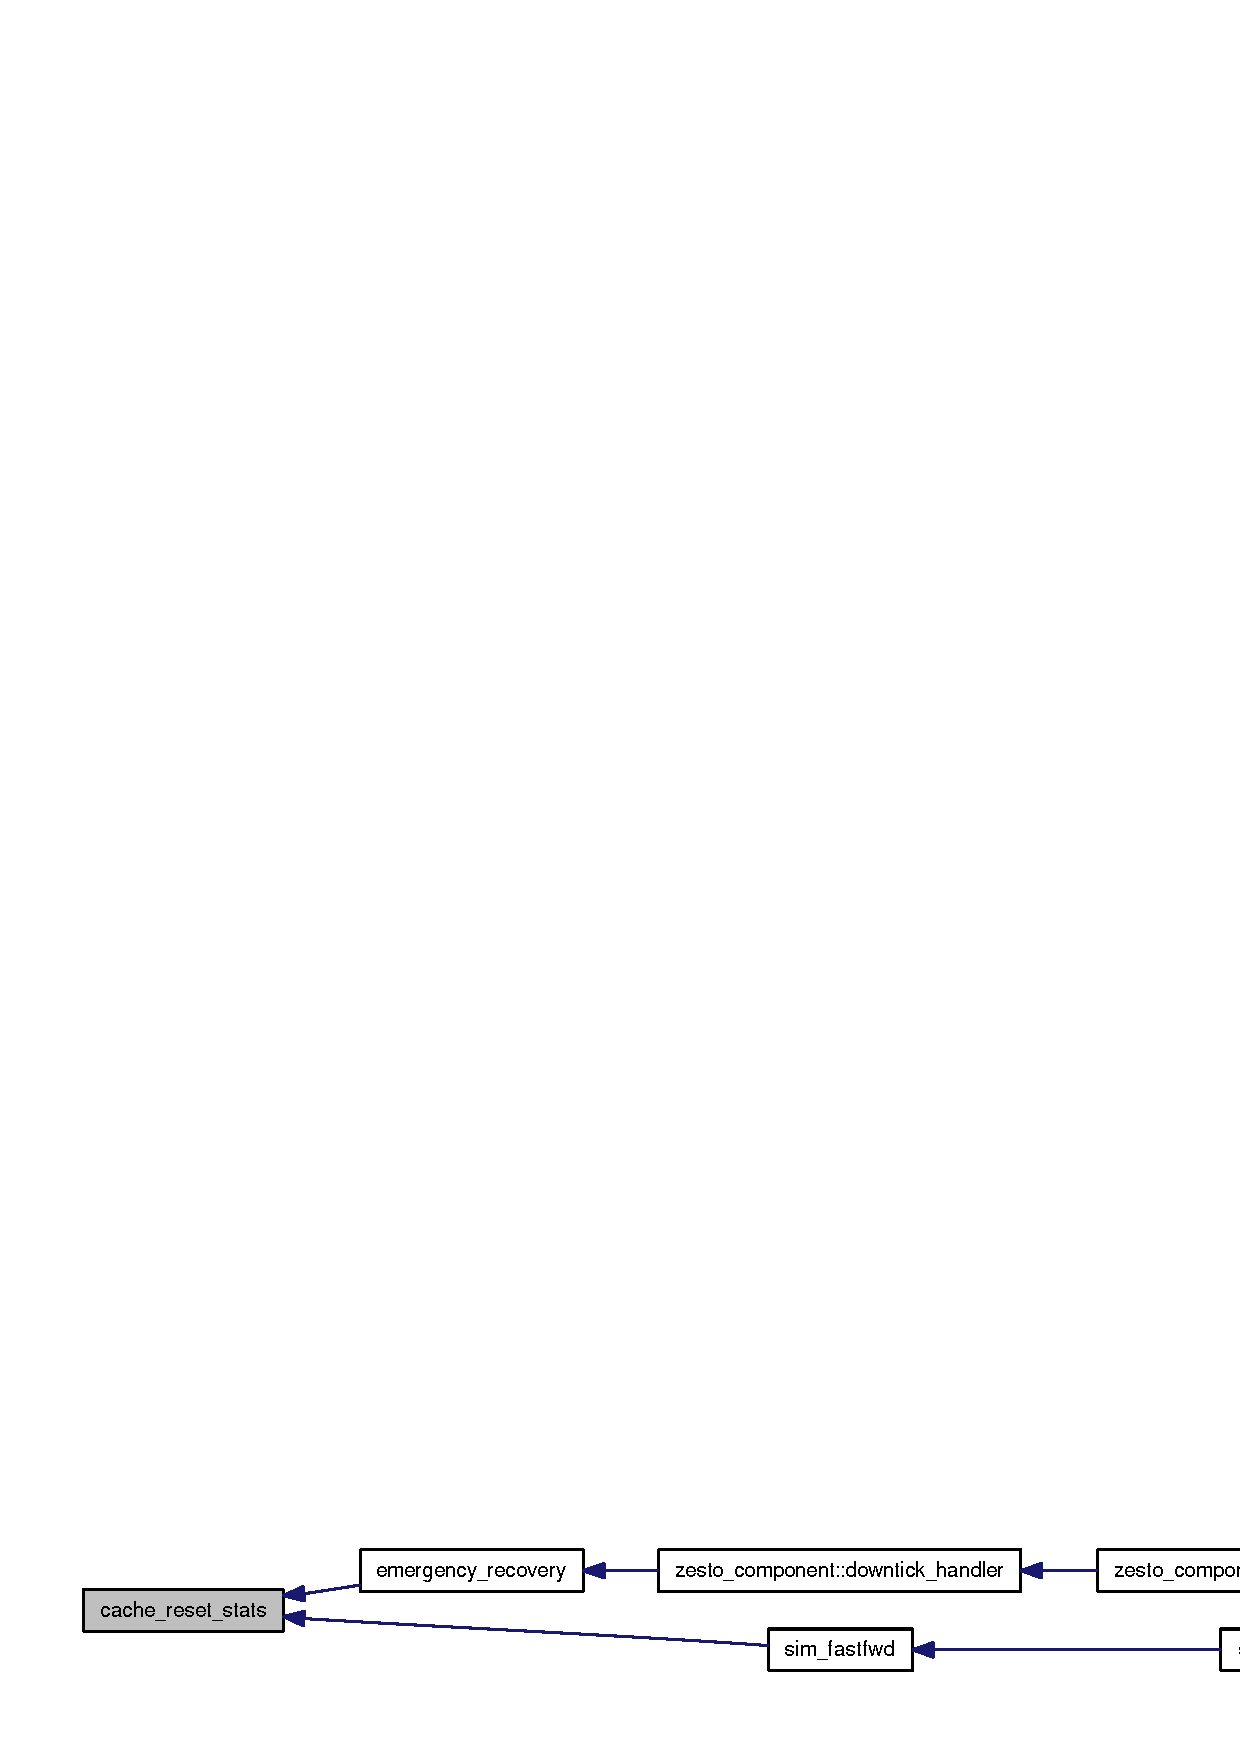
\includegraphics[width=391pt]{config_2zesto-cache_8cpp_aff01697c94f19565dfd6d631bf4bf76_icgraph}
\end{center}
\end{figure}
\index{config/zesto-cache.cpp@{config/zesto-cache.cpp}!dummy\_\-callback@{dummy\_\-callback}}
\index{dummy\_\-callback@{dummy\_\-callback}!config/zesto-cache.cpp@{config/zesto-cache.cpp}}
\subsubsection[{dummy\_\-callback}]{\setlength{\rightskip}{0pt plus 5cm}static void dummy\_\-callback (void $\ast$ {\em p})\hspace{0.3cm}{\tt  [static]}}\label{config_2zesto-cache_8cpp_2ca1ae8eb0053c08276d5e170a5f98d8}




Definition at line 1325 of file config/zesto-cache.cpp.

Referenced by cache\_\-prefetch(), cache\_\-prefetch\_\-llc(), and cache\_\-process().

Here is the caller graph for this function:\nopagebreak
\begin{figure}[H]
\begin{center}
\leavevmode
\includegraphics[width=420pt]{config_2zesto-cache_8cpp_2ca1ae8eb0053c08276d5e170a5f98d8_icgraph}
\end{center}
\end{figure}
\index{config/zesto-cache.cpp@{config/zesto-cache.cpp}!fill\_\-arrived@{fill\_\-arrived}}
\index{fill\_\-arrived@{fill\_\-arrived}!config/zesto-cache.cpp@{config/zesto-cache.cpp}}
\subsubsection[{fill\_\-arrived}]{\setlength{\rightskip}{0pt plus 5cm}void fill\_\-arrived (struct {\bf cache\_\-t} $\ast$const  {\em cp}, \/  const int {\em MSHR\_\-bank}, \/  const int {\em MSHR\_\-index})}\label{config_2zesto-cache_8cpp_4d5f99649851ca3db130a4a6228a1f35}




Definition at line 1333 of file config/zesto-cache.cpp.

Referenced by cache\_\-process(), and cache\_\-process\_\-llc().

Here is the caller graph for this function:\nopagebreak
\begin{figure}[H]
\begin{center}
\leavevmode
\includegraphics[width=214pt]{config_2zesto-cache_8cpp_4d5f99649851ca3db130a4a6228a1f35_icgraph}
\end{center}
\end{figure}
\index{config/zesto-cache.cpp@{config/zesto-cache.cpp}!fill\_\-heap\_\-balance@{fill\_\-heap\_\-balance}}
\index{fill\_\-heap\_\-balance@{fill\_\-heap\_\-balance}!config/zesto-cache.cpp@{config/zesto-cache.cpp}}
\subsubsection[{fill\_\-heap\_\-balance}]{\setlength{\rightskip}{0pt plus 5cm}static void fill\_\-heap\_\-balance (struct {\bf cache\_\-fill\_\-t} $\ast$const  {\em pipe}, \/  const int {\em insert\_\-position})\hspace{0.3cm}{\tt  [static]}}\label{config_2zesto-cache_8cpp_45008d7fc6cedc3c5187a70e4cfc1d4a}




Definition at line 1383 of file config/zesto-cache.cpp.

References memswap(), and cache\_\-action\_\-t::pipe\_\-exit\_\-time.

Referenced by cache\_\-fill(), and cache\_\-fill\_\-llc().

Here is the caller graph for this function:\nopagebreak
\begin{figure}[H]
\begin{center}
\leavevmode
\includegraphics[width=284pt]{config_2zesto-cache_8cpp_45008d7fc6cedc3c5187a70e4cfc1d4a_icgraph}
\end{center}
\end{figure}
\index{config/zesto-cache.cpp@{config/zesto-cache.cpp}!fill\_\-heap\_\-remove@{fill\_\-heap\_\-remove}}
\index{fill\_\-heap\_\-remove@{fill\_\-heap\_\-remove}!config/zesto-cache.cpp@{config/zesto-cache.cpp}}
\subsubsection[{fill\_\-heap\_\-remove}]{\setlength{\rightskip}{0pt plus 5cm}static void fill\_\-heap\_\-remove (struct {\bf cache\_\-fill\_\-t} $\ast$const  {\em pipe}, \/  const int {\em pipe\_\-num})\hspace{0.3cm}{\tt  [static]}}\label{config_2zesto-cache_8cpp_9c8931eb6f26a4862221d39dd688368f}




Definition at line 1407 of file config/zesto-cache.cpp.

References memswap(), cache\_\-fill\_\-t::pipe\_\-exit\_\-time, TICK\_\-T\_\-MAX, and cache\_\-fill\_\-t::valid.

Referenced by cache\_\-process(), and cache\_\-process\_\-llc().

Here is the caller graph for this function:\nopagebreak
\begin{figure}[H]
\begin{center}
\leavevmode
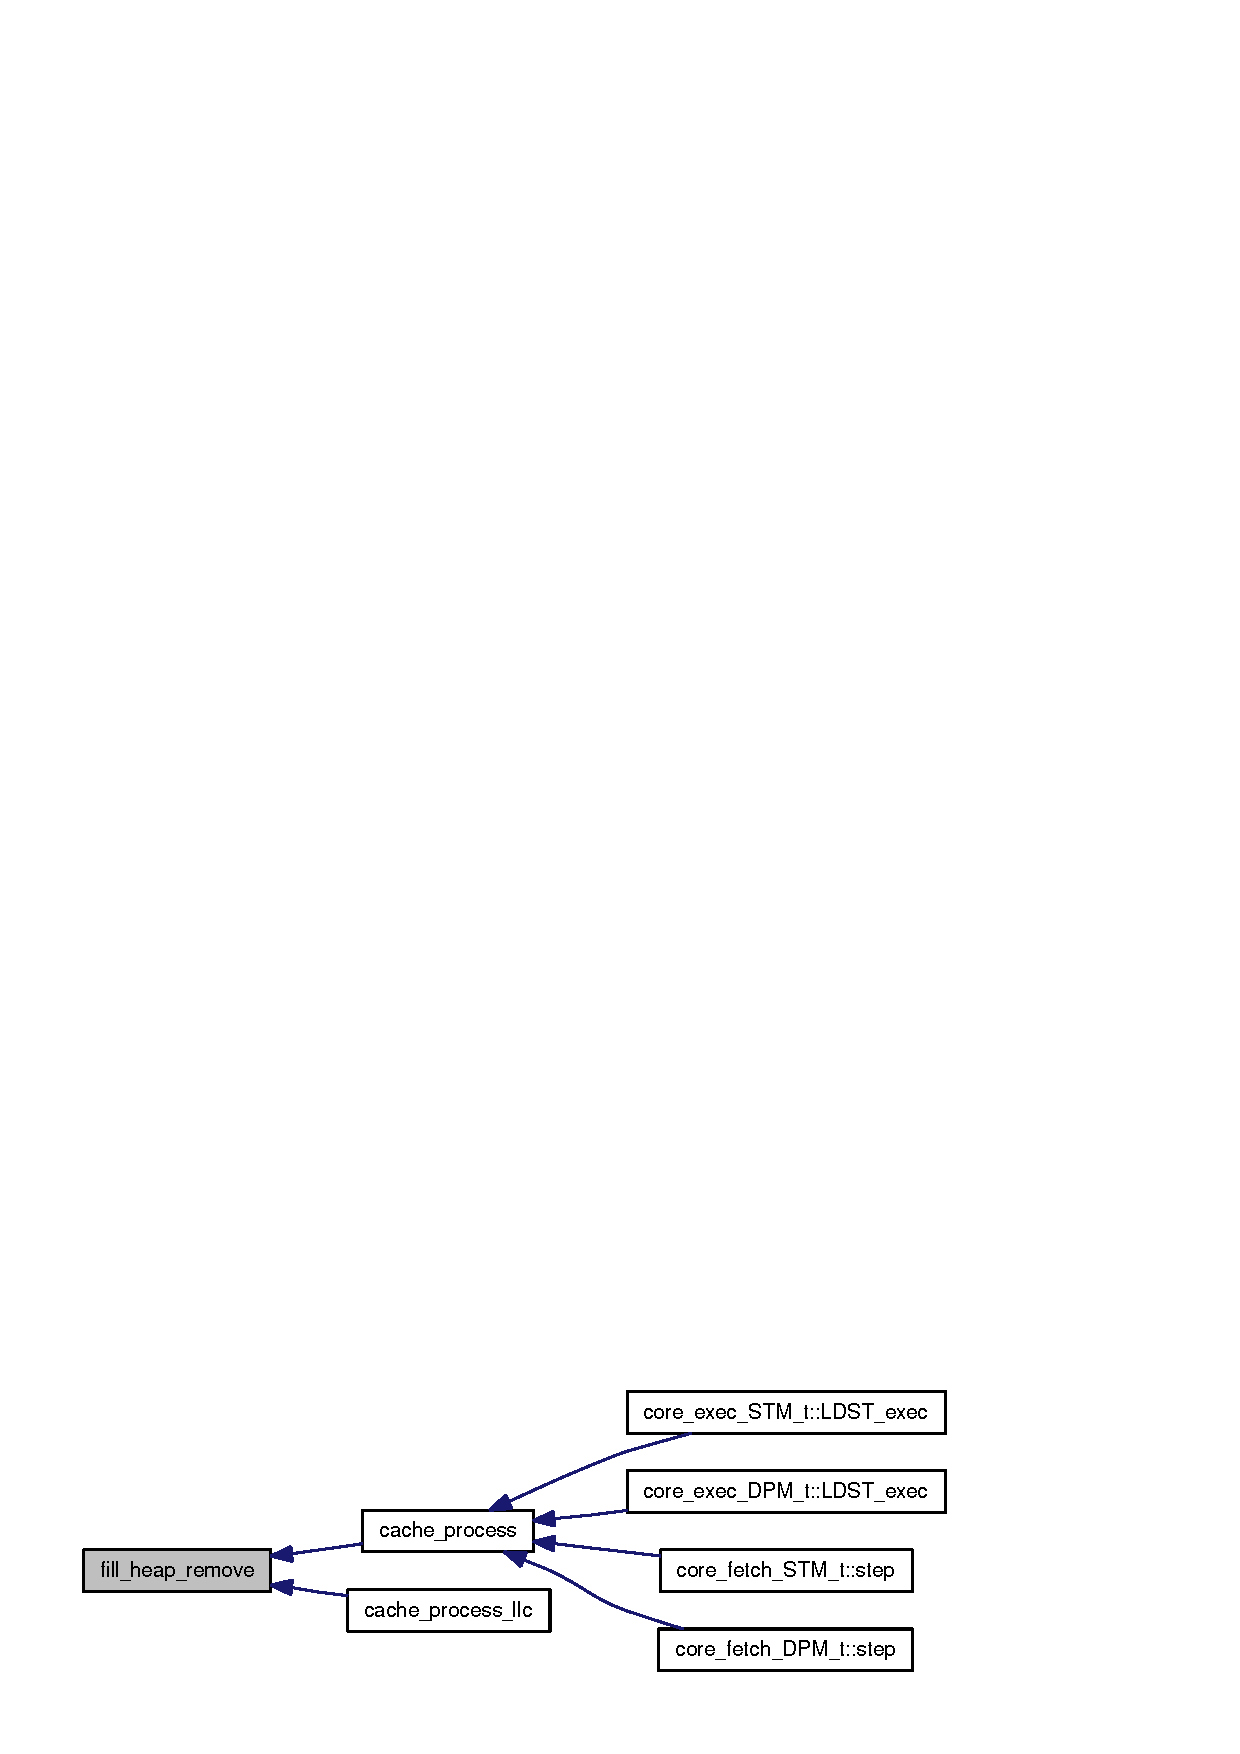
\includegraphics[width=229pt]{config_2zesto-cache_8cpp_9c8931eb6f26a4862221d39dd688368f_icgraph}
\end{center}
\end{figure}
\index{config/zesto-cache.cpp@{config/zesto-cache.cpp}!MSHR\_\-allocate@{MSHR\_\-allocate}}
\index{MSHR\_\-allocate@{MSHR\_\-allocate}!config/zesto-cache.cpp@{config/zesto-cache.cpp}}
\subsubsection[{MSHR\_\-allocate}]{\setlength{\rightskip}{0pt plus 5cm}static struct {\bf cache\_\-action\_\-t}$\ast$ MSHR\_\-allocate (struct {\bf cache\_\-t} $\ast$const  {\em cp}, \/  const {\bf md\_\-paddr\_\-t} {\em paddr}, \/  const enum {\bf cache\_\-command} {\em cmd})\hspace{0.3cm}{\tt  [static, read]}}\label{config_2zesto-cache_8cpp_b9e90f1afc77db8eb4dad712b12304ac}




Definition at line 1271 of file config/zesto-cache.cpp.

References cache\_\-t::addr\_\-shift, cache\_\-assert, cache\_\-action\_\-t::cb, cache\_\-t::check\_\-for\_\-MSHR\_\-work, cache\_\-t::check\_\-for\_\-work, fatal(), GET\_\-MSHR\_\-BANK, cache\_\-t::MSHR, cache\_\-t::MSHR\_\-combos, cache\_\-action\_\-t::MSHR\_\-link, cache\_\-action\_\-t::MSHR\_\-linked, cache\_\-t::MSHR\_\-size, cache\_\-action\_\-t::paddr, cache\_\-t::stat, TICK\_\-T\_\-MAX, and cache\_\-action\_\-t::when\_\-returned.

Referenced by cache\_\-process(), and cache\_\-process\_\-llc().

Here is the caller graph for this function:\nopagebreak
\begin{figure}[H]
\begin{center}
\leavevmode
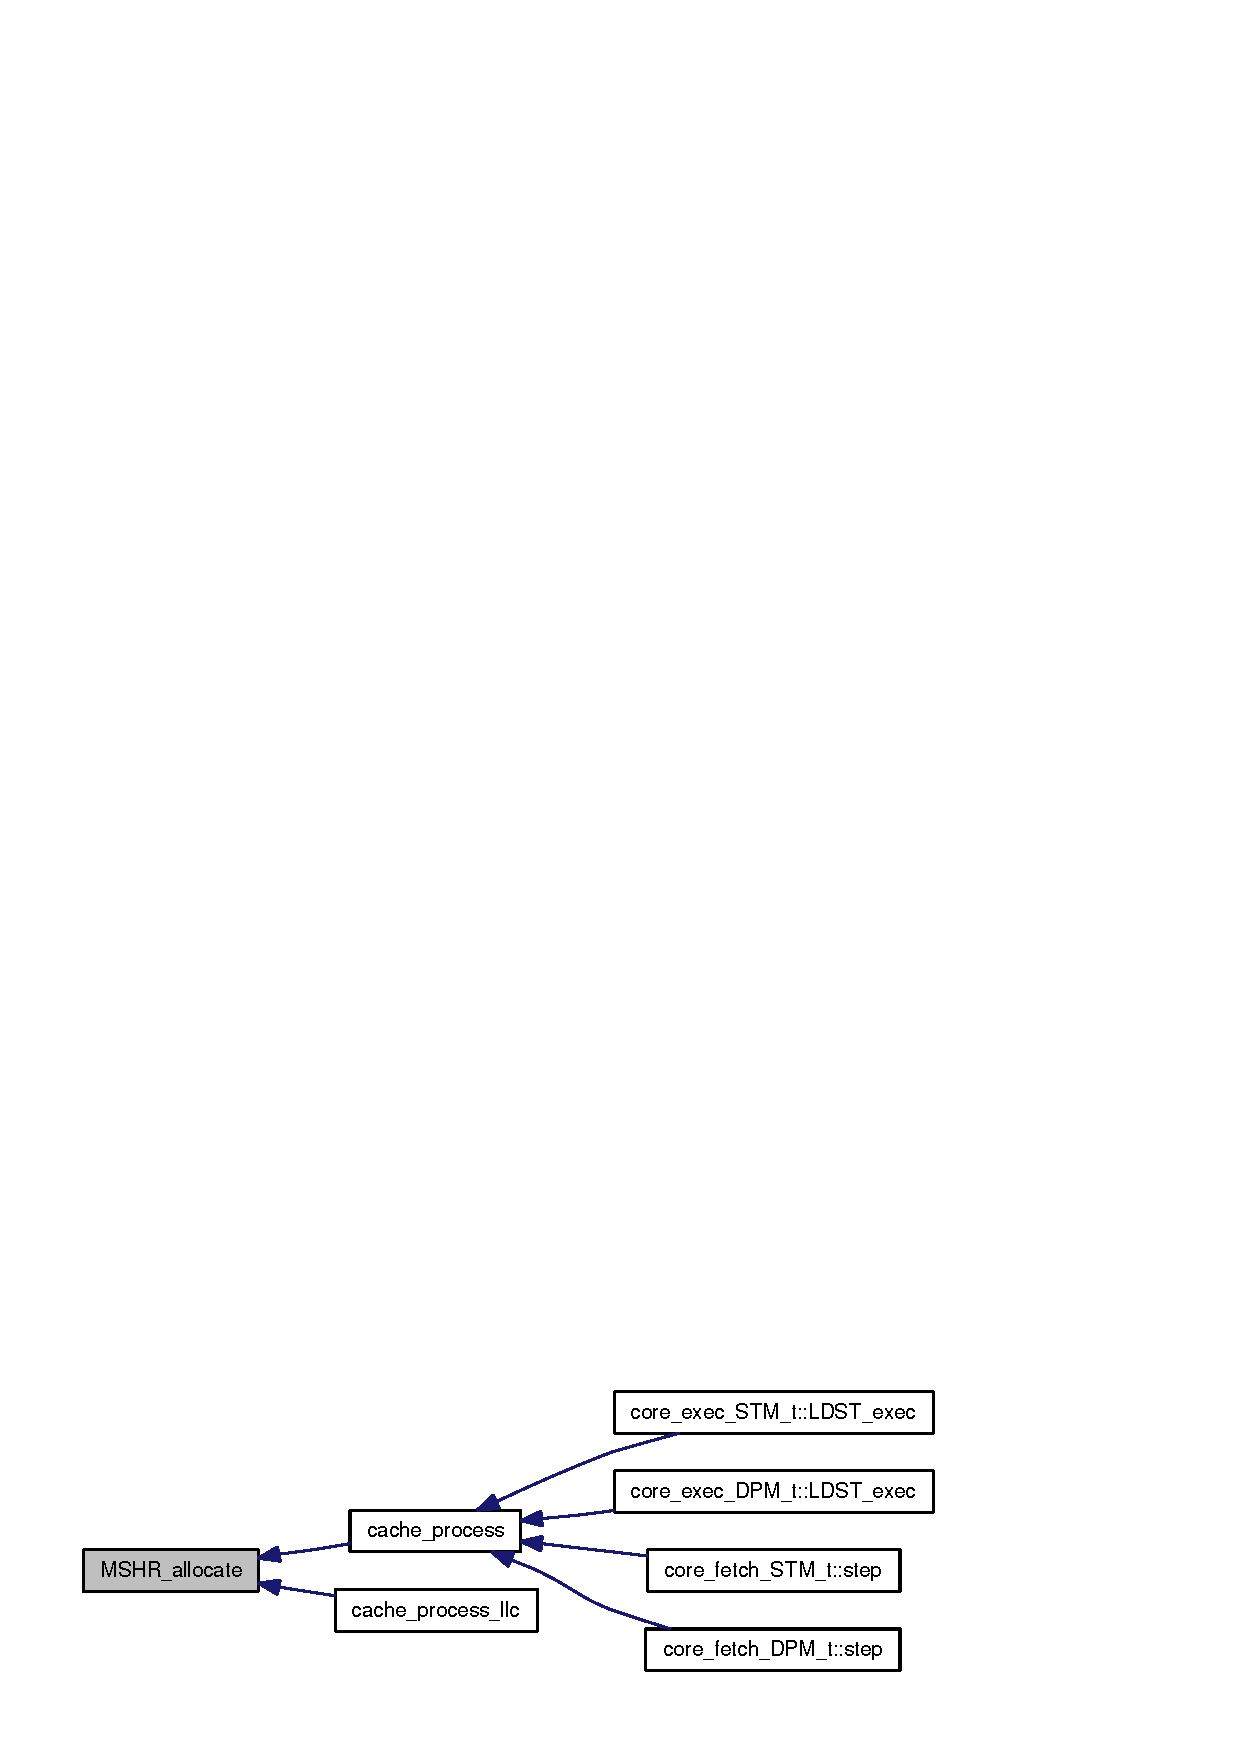
\includegraphics[width=226pt]{config_2zesto-cache_8cpp_b9e90f1afc77db8eb4dad712b12304ac_icgraph}
\end{center}
\end{figure}
\index{config/zesto-cache.cpp@{config/zesto-cache.cpp}!MSHR\_\-available@{MSHR\_\-available}}
\index{MSHR\_\-available@{MSHR\_\-available}!config/zesto-cache.cpp@{config/zesto-cache.cpp}}
\subsubsection[{MSHR\_\-available}]{\setlength{\rightskip}{0pt plus 5cm}static int MSHR\_\-available (const struct {\bf cache\_\-t} $\ast$const  {\em cp}, \/  const {\bf md\_\-paddr\_\-t} {\em paddr})\hspace{0.3cm}{\tt  [inline, static]}}\label{config_2zesto-cache_8cpp_eb1b85c3ab5d1ac1520577d21fd09dee}




Definition at line 1261 of file config/zesto-cache.cpp.

References GET\_\-MSHR\_\-BANK, and cache\_\-t::MSHR\_\-size.

Referenced by cache\_\-process(), and cache\_\-process\_\-llc().

Here is the caller graph for this function:\nopagebreak
\begin{figure}[H]
\begin{center}
\leavevmode
\includegraphics[width=228pt]{config_2zesto-cache_8cpp_eb1b85c3ab5d1ac1520577d21fd09dee_icgraph}
\end{center}
\end{figure}
\index{config/zesto-cache.cpp@{config/zesto-cache.cpp}!prefetch\_\-buffer\_\-create@{prefetch\_\-buffer\_\-create}}
\index{prefetch\_\-buffer\_\-create@{prefetch\_\-buffer\_\-create}!config/zesto-cache.cpp@{config/zesto-cache.cpp}}
\subsubsection[{prefetch\_\-buffer\_\-create}]{\setlength{\rightskip}{0pt plus 5cm}void prefetch\_\-buffer\_\-create (struct {\bf cache\_\-t} $\ast$const  {\em cp}, \/  const int {\em num\_\-entries})}\label{config_2zesto-cache_8cpp_16dacff1f1e08b2a7fe82d35f3733f91}




Definition at line 531 of file config/zesto-cache.cpp.

Referenced by core\_\-exec\_\-DPM\_\-t::core\_\-exec\_\-DPM\_\-t(), core\_\-fetch\_\-DPM\_\-t::core\_\-fetch\_\-DPM\_\-t(), and uncore\_\-t::uncore\_\-t().

Here is the caller graph for this function:\nopagebreak
\begin{figure}[H]
\begin{center}
\leavevmode
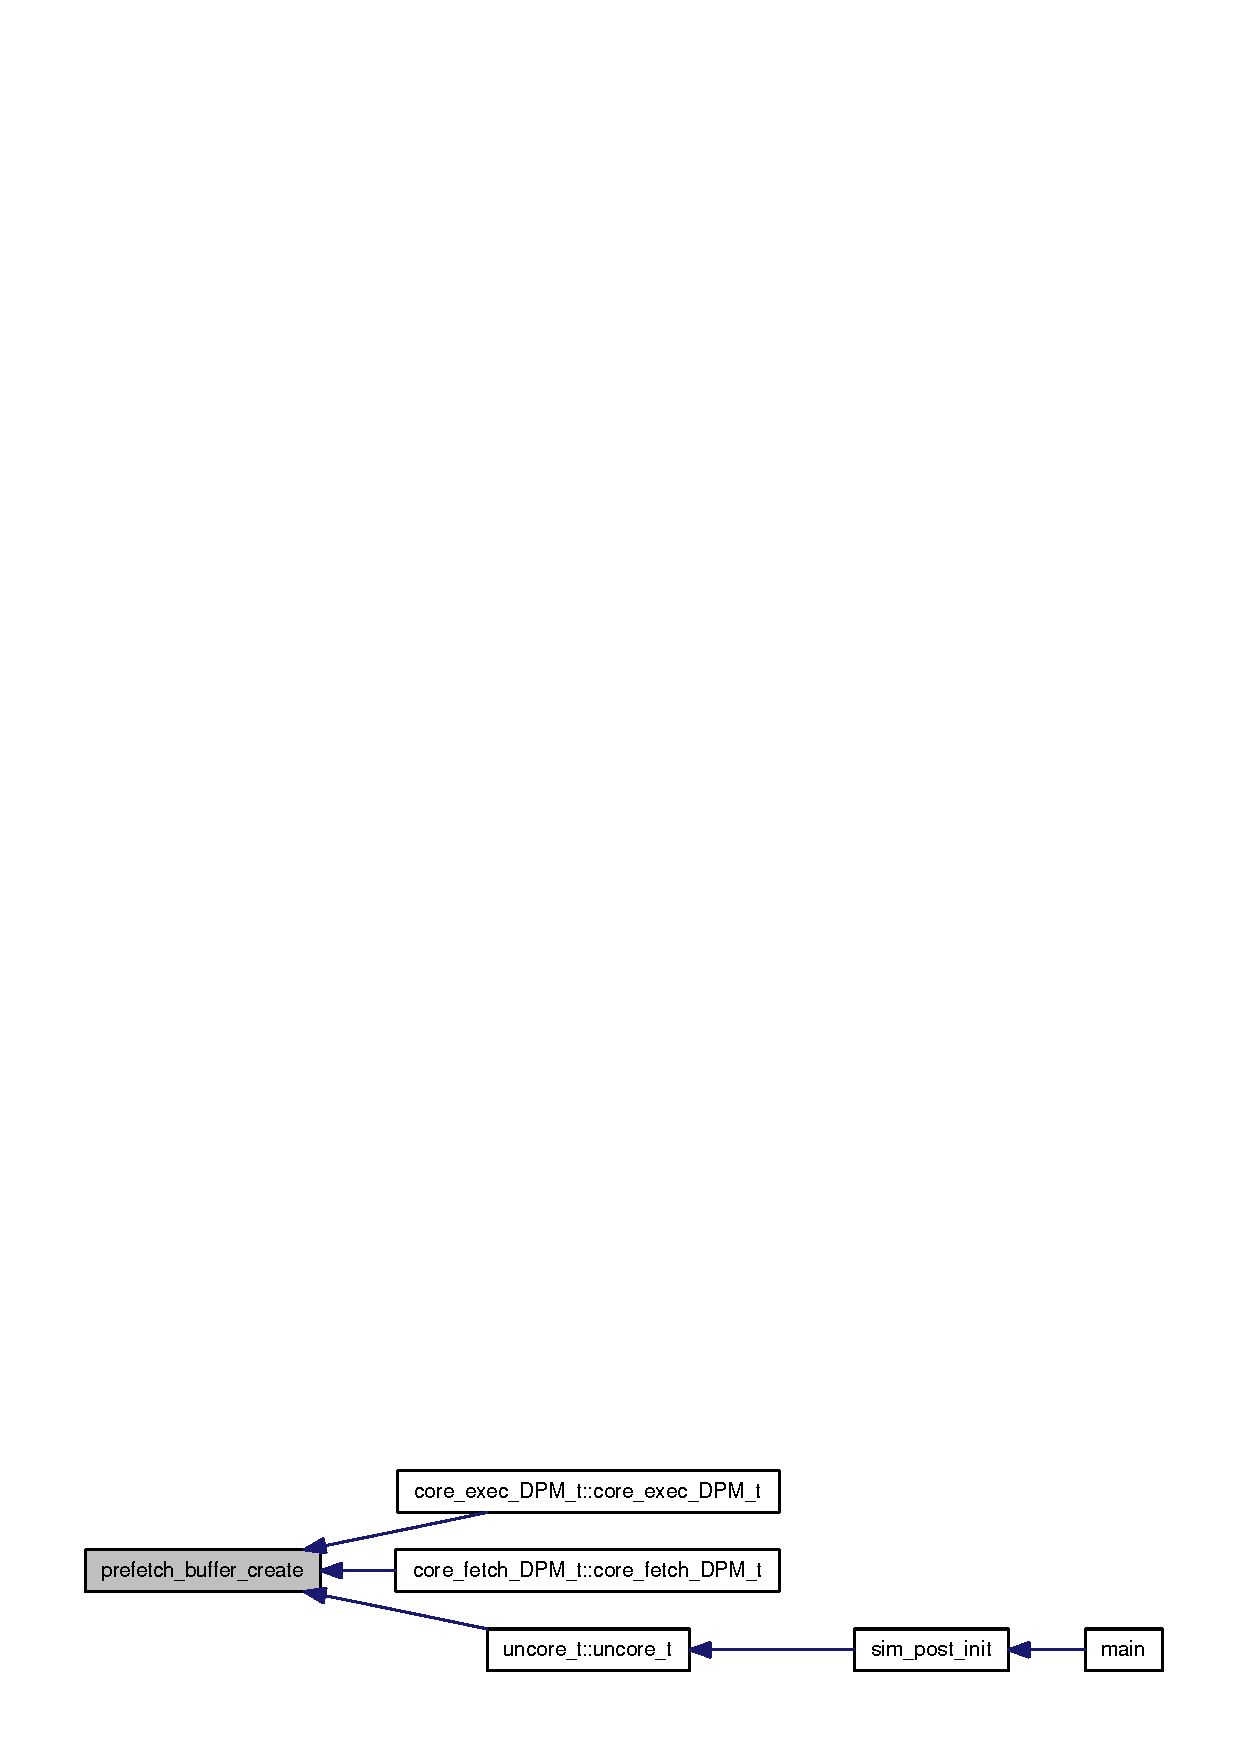
\includegraphics[width=281pt]{config_2zesto-cache_8cpp_16dacff1f1e08b2a7fe82d35f3733f91_icgraph}
\end{center}
\end{figure}
\index{config/zesto-cache.cpp@{config/zesto-cache.cpp}!prefetch\_\-controller\_\-update@{prefetch\_\-controller\_\-update}}
\index{prefetch\_\-controller\_\-update@{prefetch\_\-controller\_\-update}!config/zesto-cache.cpp@{config/zesto-cache.cpp}}
\subsubsection[{prefetch\_\-controller\_\-update}]{\setlength{\rightskip}{0pt plus 5cm}static void prefetch\_\-controller\_\-update (struct {\bf cache\_\-t} $\ast$const  {\em cp})\hspace{0.3cm}{\tt  [static]}}\label{config_2zesto-cache_8cpp_563b4fe087e7d8225f1e3aea2f1e8235}




Definition at line 2372 of file config/zesto-cache.cpp.

References cache\_\-t::next\_\-bus, cache\_\-t::PF\_\-high\_\-watermark, cache\_\-t::PF\_\-last\_\-sample, PF\_\-OK, PF\_\-REFRAIN, cache\_\-t::PF\_\-sample\_\-interval, cache\_\-t::PF\_\-state, sim\_\-cycle, bus\_\-t::stat, and bus\_\-t::utilization.

Referenced by step\_\-core\_\-PF\_\-controllers().

Here is the caller graph for this function:\nopagebreak
\begin{figure}[H]
\begin{center}
\leavevmode
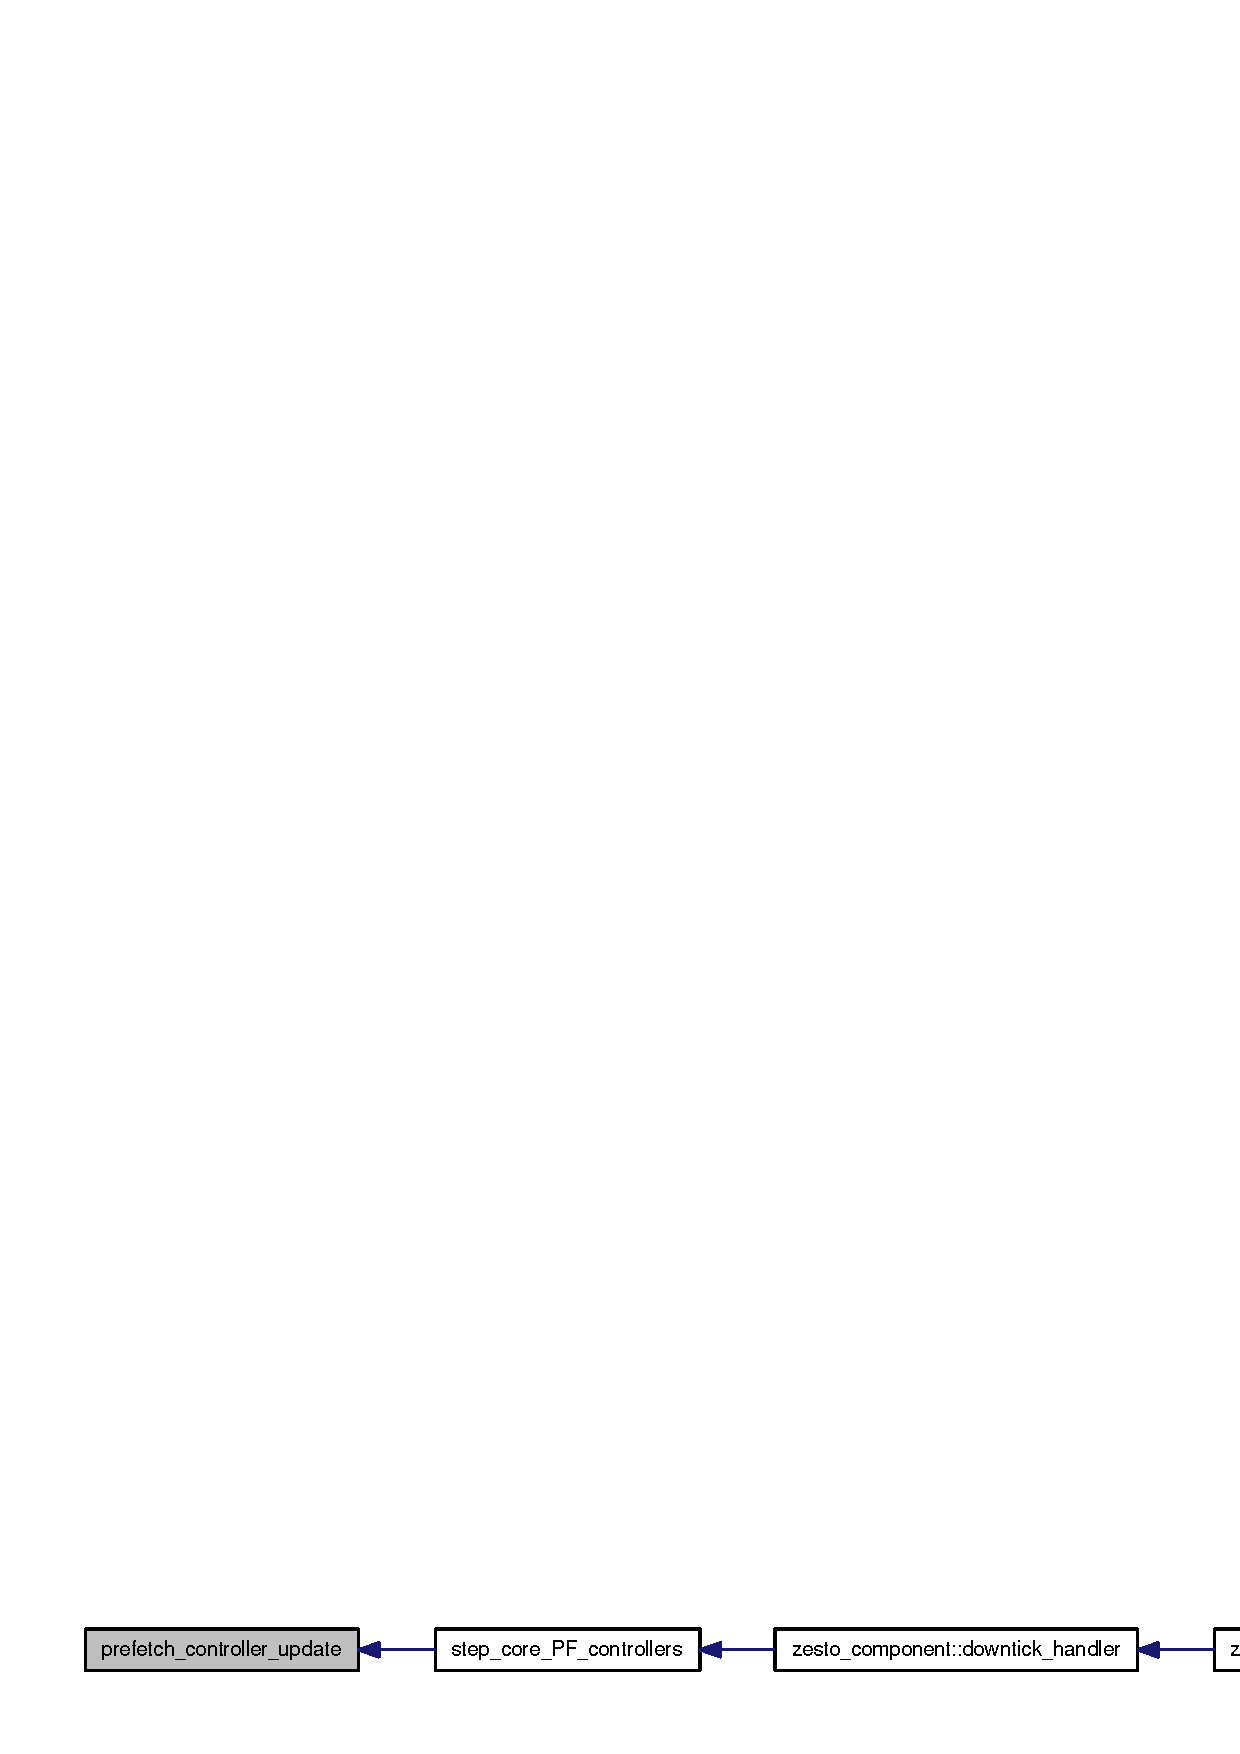
\includegraphics[width=419pt]{config_2zesto-cache_8cpp_563b4fe087e7d8225f1e3aea2f1e8235_icgraph}
\end{center}
\end{figure}
\index{config/zesto-cache.cpp@{config/zesto-cache.cpp}!prefetch\_\-core\_\-caches@{prefetch\_\-core\_\-caches}}
\index{prefetch\_\-core\_\-caches@{prefetch\_\-core\_\-caches}!config/zesto-cache.cpp@{config/zesto-cache.cpp}}
\subsubsection[{prefetch\_\-core\_\-caches}]{\setlength{\rightskip}{0pt plus 5cm}void prefetch\_\-core\_\-caches (struct {\bf core\_\-t} $\ast$const  {\em core})}\label{config_2zesto-cache_8cpp_3f3ef48df254425f422f6cf5de128ade}




Definition at line 2395 of file config/zesto-cache.cpp.

Referenced by zesto\_\-component::downtick\_\-handler().

Here is the caller graph for this function:\nopagebreak
\begin{figure}[H]
\begin{center}
\leavevmode
\includegraphics[width=327pt]{config_2zesto-cache_8cpp_3f3ef48df254425f422f6cf5de128ade_icgraph}
\end{center}
\end{figure}
\index{config/zesto-cache.cpp@{config/zesto-cache.cpp}!prefetch\_\-filter\_\-create@{prefetch\_\-filter\_\-create}}
\index{prefetch\_\-filter\_\-create@{prefetch\_\-filter\_\-create}!config/zesto-cache.cpp@{config/zesto-cache.cpp}}
\subsubsection[{prefetch\_\-filter\_\-create}]{\setlength{\rightskip}{0pt plus 5cm}void prefetch\_\-filter\_\-create (struct {\bf cache\_\-t} $\ast$const  {\em cp}, \/  const int {\em num\_\-entries}, \/  const int {\em reset\_\-interval})}\label{config_2zesto-cache_8cpp_81be4d7fbc22a3d9f3fcaa52715c22e9}




Definition at line 552 of file config/zesto-cache.cpp.

Referenced by core\_\-exec\_\-DPM\_\-t::core\_\-exec\_\-DPM\_\-t(), core\_\-fetch\_\-DPM\_\-t::core\_\-fetch\_\-DPM\_\-t(), and uncore\_\-t::uncore\_\-t().

Here is the caller graph for this function:\nopagebreak
\begin{figure}[H]
\begin{center}
\leavevmode
\includegraphics[width=278pt]{config_2zesto-cache_8cpp_81be4d7fbc22a3d9f3fcaa52715c22e9_icgraph}
\end{center}
\end{figure}
\index{config/zesto-cache.cpp@{config/zesto-cache.cpp}!prefetch\_\-filter\_\-lookup@{prefetch\_\-filter\_\-lookup}}
\index{prefetch\_\-filter\_\-lookup@{prefetch\_\-filter\_\-lookup}!config/zesto-cache.cpp@{config/zesto-cache.cpp}}
\subsubsection[{prefetch\_\-filter\_\-lookup}]{\setlength{\rightskip}{0pt plus 5cm}static int prefetch\_\-filter\_\-lookup (struct {\bf prefetch\_\-filter\_\-t} $\ast$const  {\em p}, \/  const {\bf md\_\-paddr\_\-t} {\em addr})\hspace{0.3cm}{\tt  [static]}}\label{config_2zesto-cache_8cpp_17dbb4e8d2ae84f22541bef1c04253de}




Definition at line 574 of file config/zesto-cache.cpp.

References prefetch\_\-filter\_\-t::last\_\-reset, prefetch\_\-filter\_\-t::mask, prefetch\_\-filter\_\-t::num\_\-entries, prefetch\_\-filter\_\-t::reset\_\-interval, sim\_\-cycle, and prefetch\_\-filter\_\-t::table.

Referenced by cache\_\-process(), and cache\_\-process\_\-llc().

Here is the caller graph for this function:\nopagebreak
\begin{figure}[H]
\begin{center}
\leavevmode
\includegraphics[width=239pt]{config_2zesto-cache_8cpp_17dbb4e8d2ae84f22541bef1c04253de_icgraph}
\end{center}
\end{figure}
\index{config/zesto-cache.cpp@{config/zesto-cache.cpp}!prefetch\_\-filter\_\-update@{prefetch\_\-filter\_\-update}}
\index{prefetch\_\-filter\_\-update@{prefetch\_\-filter\_\-update}!config/zesto-cache.cpp@{config/zesto-cache.cpp}}
\subsubsection[{prefetch\_\-filter\_\-update}]{\setlength{\rightskip}{0pt plus 5cm}static void prefetch\_\-filter\_\-update (struct {\bf prefetch\_\-filter\_\-t} $\ast$const  {\em p}, \/  const {\bf md\_\-paddr\_\-t} {\em addr}, \/  const int {\em useful})\hspace{0.3cm}{\tt  [static]}}\label{config_2zesto-cache_8cpp_7867a082122e5a85b7e880d3bfb243f9}




Definition at line 591 of file config/zesto-cache.cpp.

References prefetch\_\-filter\_\-t::last\_\-reset, prefetch\_\-filter\_\-t::mask, prefetch\_\-filter\_\-t::num\_\-entries, prefetch\_\-filter\_\-t::reset\_\-interval, sim\_\-cycle, and prefetch\_\-filter\_\-t::table.

Referenced by cache\_\-process(), and cache\_\-process\_\-llc().

Here is the caller graph for this function:\nopagebreak
\begin{figure}[H]
\begin{center}
\leavevmode
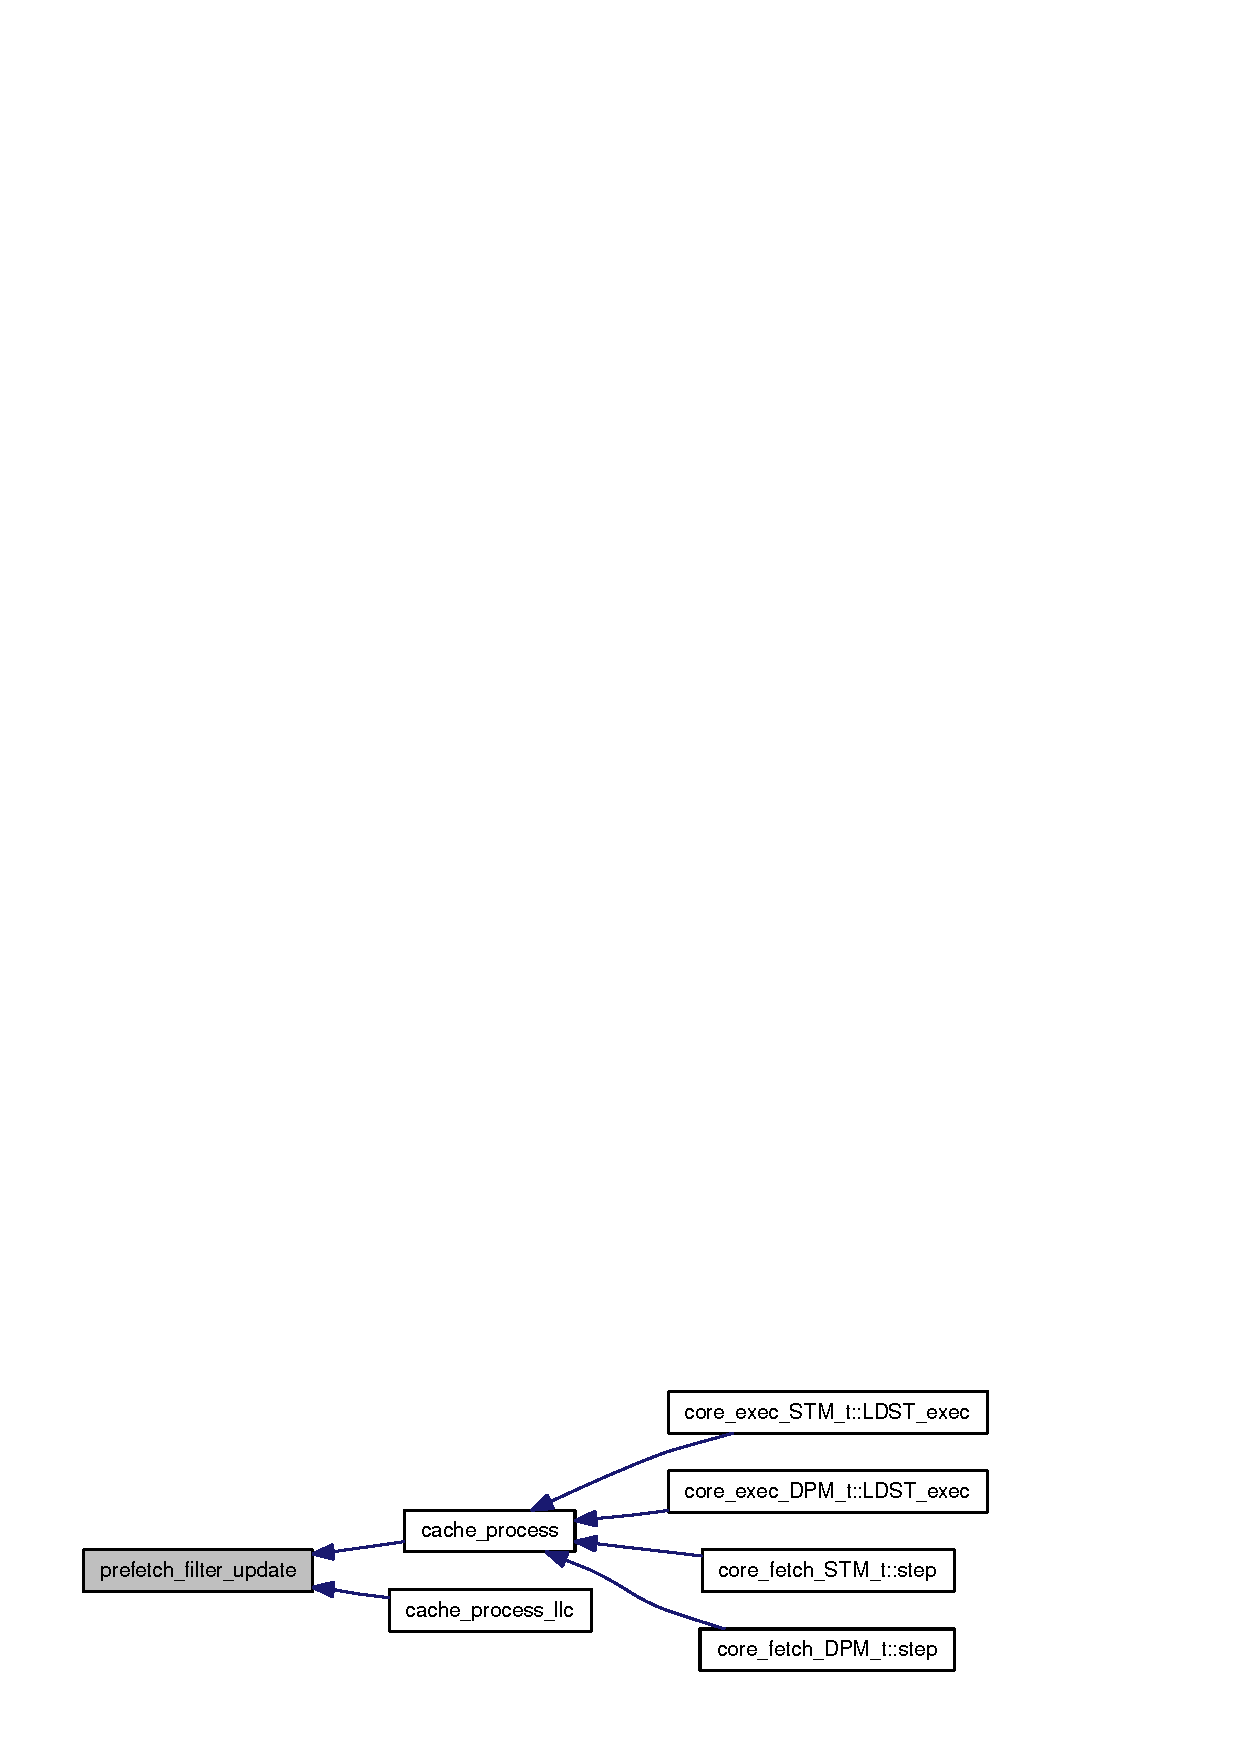
\includegraphics[width=239pt]{config_2zesto-cache_8cpp_7867a082122e5a85b7e880d3bfb243f9_icgraph}
\end{center}
\end{figure}
\index{config/zesto-cache.cpp@{config/zesto-cache.cpp}!print\_\-heap@{print\_\-heap}}
\index{print\_\-heap@{print\_\-heap}!config/zesto-cache.cpp@{config/zesto-cache.cpp}}
\subsubsection[{print\_\-heap}]{\setlength{\rightskip}{0pt plus 5cm}void print\_\-heap (const struct {\bf cache\_\-t} $\ast$const  {\em cp})}\label{config_2zesto-cache_8cpp_85af5d6eb3231dd22e161c347a5fd72b}




Definition at line 1367 of file config/zesto-cache.cpp.

References cache\_\-t::banks, cache\_\-t::name, cache\_\-t::pipe, cache\_\-action\_\-t::pipe\_\-exit\_\-time, and cache\_\-t::pipe\_\-num.\index{config/zesto-cache.cpp@{config/zesto-cache.cpp}!step\_\-core\_\-PF\_\-controllers@{step\_\-core\_\-PF\_\-controllers}}
\index{step\_\-core\_\-PF\_\-controllers@{step\_\-core\_\-PF\_\-controllers}!config/zesto-cache.cpp@{config/zesto-cache.cpp}}
\subsubsection[{step\_\-core\_\-PF\_\-controllers}]{\setlength{\rightskip}{0pt plus 5cm}void step\_\-core\_\-PF\_\-controllers (struct {\bf core\_\-t} $\ast$const  {\em core})}\label{config_2zesto-cache_8cpp_66309167ab5b4ca25ad2bfbf94b0126b}




Definition at line 2387 of file config/zesto-cache.cpp.

Referenced by zesto\_\-component::downtick\_\-handler().

Here is the caller graph for this function:\nopagebreak
\begin{figure}[H]
\begin{center}
\leavevmode
\includegraphics[width=335pt]{config_2zesto-cache_8cpp_66309167ab5b4ca25ad2bfbf94b0126b_icgraph}
\end{center}
\end{figure}
\index{config/zesto-cache.cpp@{config/zesto-cache.cpp}!WBB\_\-available@{WBB\_\-available}}
\index{WBB\_\-available@{WBB\_\-available}!config/zesto-cache.cpp@{config/zesto-cache.cpp}}
\subsubsection[{WBB\_\-available}]{\setlength{\rightskip}{0pt plus 5cm}static int WBB\_\-available (const struct {\bf cache\_\-t} $\ast$const  {\em cp}, \/  const {\bf md\_\-paddr\_\-t} {\em paddr})\hspace{0.3cm}{\tt  [inline, static]}}\label{config_2zesto-cache_8cpp_48f8188c331e3c2188868d0f1c577d5a}




Definition at line 1169 of file config/zesto-cache.cpp.

References GET\_\-MSHR\_\-BANK, cache\_\-t::WBB\_\-num, and cache\_\-t::WBB\_\-size.

Referenced by cache\_\-process(), and cache\_\-process\_\-llc().

Here is the caller graph for this function:\nopagebreak
\begin{figure}[H]
\begin{center}
\leavevmode
\includegraphics[width=225pt]{config_2zesto-cache_8cpp_48f8188c331e3c2188868d0f1c577d5a_icgraph}
\end{center}
\end{figure}
\index{config/zesto-cache.cpp@{config/zesto-cache.cpp}!WBB\_\-insert@{WBB\_\-insert}}
\index{WBB\_\-insert@{WBB\_\-insert}!config/zesto-cache.cpp@{config/zesto-cache.cpp}}
\subsubsection[{WBB\_\-insert}]{\setlength{\rightskip}{0pt plus 5cm}static void WBB\_\-insert (struct {\bf cache\_\-t} $\ast$const  {\em cp}, \/  struct {\bf cache\_\-line\_\-t} $\ast$const  {\em cache\_\-block})\hspace{0.3cm}{\tt  [static]}}\label{config_2zesto-cache_8cpp_54a68443796a201ceb5456ce0fc69bc4}




Definition at line 1179 of file config/zesto-cache.cpp.

References cache\_\-t::addr\_\-shift, cache\_\-assert, CACHE\_\-STAT, cache\_\-t::check\_\-for\_\-WBB\_\-work, cache\_\-t::check\_\-for\_\-work, cache\_\-line\_\-t::core, cache\_\-line\_\-t::dirty, GET\_\-MSHR\_\-BANK, mod2m(), modinc(), cache\_\-t::stat, cache\_\-line\_\-t::tag, cache\_\-line\_\-t::valid, cache\_\-line\_\-t::victim, cache\_\-t::WBB, cache\_\-t::WBB\_\-combines, cache\_\-t::WBB\_\-head, cache\_\-t::WBB\_\-insertions, cache\_\-t::WBB\_\-num, cache\_\-t::WBB\_\-size, cache\_\-t::WBB\_\-tail, and cache\_\-t::write\_\-combining.

Referenced by cache\_\-process(), and cache\_\-process\_\-llc().

Here is the caller graph for this function:\nopagebreak
\begin{figure}[H]
\begin{center}
\leavevmode
\includegraphics[width=218pt]{config_2zesto-cache_8cpp_54a68443796a201ceb5456ce0fc69bc4_icgraph}
\end{center}
\end{figure}
\index{config/zesto-cache.cpp@{config/zesto-cache.cpp}!WBB\_\-victim\_\-insert@{WBB\_\-victim\_\-insert}}
\index{WBB\_\-victim\_\-insert@{WBB\_\-victim\_\-insert}!config/zesto-cache.cpp@{config/zesto-cache.cpp}}
\subsubsection[{WBB\_\-victim\_\-insert}]{\setlength{\rightskip}{0pt plus 5cm}static void WBB\_\-victim\_\-insert (struct {\bf cache\_\-t} $\ast$const  {\em cp}, \/  struct {\bf cache\_\-line\_\-t} $\ast$const  {\em cache\_\-block})\hspace{0.3cm}{\tt  [static]}}\label{config_2zesto-cache_8cpp_4a2ea45f307de25eaffcd48354e67a18}




Definition at line 1222 of file config/zesto-cache.cpp.

References cache\_\-t::addr\_\-shift, cache\_\-assert, CACHE\_\-STAT, cache\_\-line\_\-t::core, cache\_\-line\_\-t::dirty, GET\_\-MSHR\_\-BANK, mod2m(), cache\_\-t::stat, cache\_\-line\_\-t::tag, cache\_\-line\_\-t::valid, cache\_\-line\_\-t::victim, cache\_\-t::WBB, cache\_\-t::WBB\_\-head, cache\_\-t::WBB\_\-num, cache\_\-t::WBB\_\-size, and cache\_\-t::WBB\_\-victim\_\-insertions.

Referenced by cache\_\-process().

Here is the caller graph for this function:\nopagebreak
\begin{figure}[H]
\begin{center}
\leavevmode
\includegraphics[width=226pt]{config_2zesto-cache_8cpp_4a2ea45f307de25eaffcd48354e67a18_icgraph}
\end{center}
\end{figure}
